\documentclass[11pt, oneside, ngerman]{report}

\usepackage[utf8]{inputenc}
\usepackage[T1]{fontenc}
\usepackage[ngerman]{babel}
\usepackage{config/style}
\usepackage{config/code}
\usepackage{glossaries}
\usepackage{biblatex}
\usepackage{booktabs}
\usepackage{array}
\usepackage{amsmath}
\usepackage{tikz}
\usetikzlibrary{shapes.geometric, arrows.meta, positioning, chains, decorations.pathmorphing, patterns}

\addbibresource{references.bib}
\loadglsentries{glossar.tex}

\makeglossaries

\begin{document}

    \newcommand{\paperauthor}{Eric Seidel}
\newcommand{\papersupervisor}{Prof. Luis}
\newcommand{\paperuniversity}{Westfälische Hochschule}

\newcommand{\papertitle}{OPR Semesterzusammenfassung}
\newcommand{\papermajorheading}{OPR}
\newcommand{\paperminorheading}{Alles wichtige auf einen Blick}
    \begin{titlepage}

\newcommand{\HRule}{\rule{\linewidth}{0.5mm}} % Defines a new command for the horizontal lines, change thickness here

\center % Center everything on the page

%----------------------------------------------------------------------------------------
%	HEADING SECTIONS
%----------------------------------------------------------------------------------------

\textsc{\LARGE \paperuniversity}\\[1.0cm] % Name of your university/college
\textsc{\Large \papermajorheading}\\[0.2cm] % Major heading such as course name
\textsc{\large \paperminorheading}\\[0.75cm] % Minor heading such as course title

%----------------------------------------------------------------------------------------
%	TITLE SECTION
%----------------------------------------------------------------------------------------

\HRule \\[0.4cm]
{ \huge \bfseries \papertitle}\\[0.05cm] % Title of your document
\HRule \\[3.5cm]

\begin{center}
	\makebox[0.8\textwidth]{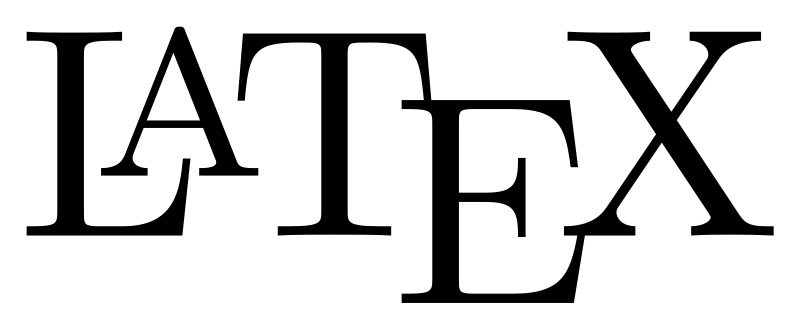
\includegraphics[width=0.8\textwidth]{frontpage.png}}
\end{center}

\vfill % Fill the rest of the page with whitespace

%----------------------------------------------------------------------------------------
%	AUTHOR SECTION
%----------------------------------------------------------------------------------------

\begin{minipage}{0.4\textwidth}
	\begin{flushleft} \large
	\emph{Author(s):}\\
	\paperauthor
	\end{flushleft}
	\end{minipage}
	~
	\begin{minipage}{0.4\textwidth}
	\begin{flushright} \large
	\emph{Supervisor(s):} \\
	\papersupervisor
	\end{flushright}
\end{minipage}\\[1cm]

%----------------------------------------------------------------------------------------
%	DATE SECTION
%----------------------------------------------------------------------------------------

{\large \today}\\ % Date, change the \today to a set date if you want to be precise

\end{titlepage}


    \clearpage
    \thispagestyle{empty}
    \pagenumbering{gobble}

    \renewcommand{\abstractname}{Copyright \textcopyright \xspace \the\year \xspace \paperuniversity}

% \begin{abstract}
\begin{center}

This document, including appendices, is property of \paperuniversity \xspace and is confidential, privileged and only for use of the intended addressees and may not be used, published or redistributed without the prior written consent of \paperuniversity \xspace.

\end{center}
% \end{abstract}

    \renewcommand{\abstractname}{Abstract}

\begin{abstract}
\begin{center}

Lorem ipsum dolor sit amet, consectetur adipiscing elit. Nam a orci ornare nibh tincidunt molestie sed nec tellus. Morbi non sapien id lorem posuere pretium. Vestibulum commodo cursus purus, a elementum sem imperdiet sit amet. Phasellus posuere dolor dignissim aliquam tempus. Morbi egestas felis in lorem varius, ac egestas ante lacinia. Nulla sed ultrices dui. Lorem ipsum dolor sit amet, consectetur adipiscing elit. 

\end{center}
\end{abstract}


    \clearpage
    \pagenumbering{roman} 
    \tableofcontents

    \clearpage
    \pagenumbering{arabic}

    \part{Vorlesungszusammenfassung}
    \label{part:vorlesungszusammenfassung}

    \chapter{Pakete in Java}
\label{chap:pakete}

\textit{Pakete schaffen Ordnung.} Sie bilden eine übersichtliche, hierarchische Struktur innerhalb von Java-Projekten.
Im Prinzip sind Pakete Ordnerstrukturen, die Klassen und weitere (Unter-)Pakete enthalten können.
Die Adressierung eines Paketes erfolgt durch seinen vollqualifizierten Paketpfad, der die Hierarchie widerspiegelt:
$p_1.p_2.\dots.p_n$. Dabei ist $p_n$ ein Paket innerhalb von $p_{n-1}$, welches wiederum in $p_{n-2}$ liegt, und so weiter.

Klassen werden analog dazu über ihren vollqualifizierten Namen angesprochen: $p_1.p_2.\dots.p_n.K$, wobei $K$ der Name der Klasse ist.

\begin{lstlisting}[language=Java, caption={Beispiele für Paket- und Klassenspezifikationen}, label=lst:paketbeispiele]
// Paket "regex", enthalten im Paket "util", das im Paket "java" liegt:
java.util.regex

// Klasse "StringTokenizer", enthalten im Paket "util", das im Paket "java" liegt:
java.util.StringTokenizer
\end{lstlisting}

Eine Klasse wird einem spezifischen Paket zugeordnet, indem die \texttt{package}-Anweisung als erste Zeile in der Quelldatei deklariert wird:
\begin{lstlisting}[language=Java, caption={Deklaration der Paketzugehörigkeit}]
package java.util; // Beispielhafter Paketpfad

public class Main {
  // ...
}
\end{lstlisting}
Diese Angabe ist für jede Java-Datei, die zu einem Paket gehört, obligatorisch. Vor der \texttt{package}-Anweisung dürfen lediglich Kommentare stehen
- keine anderen Klassendefinitionen, Variablen oder Importanweisungen.

\section{Importieren von Klassen und Paketen}
\label{sec:importieren}

Um Klassen aus anderen Paketen innerhalb der eigenen Klasse nutzen zu können, müssen diese \textit{importiert} werden.
Die \texttt{import}-Anweisungen stehen dabei stets am Anfang der Datei, nach der optionalen \texttt{package}-Deklaration und 
\textit{vor} dem Klassenkopf (der Klassendefinition).

In modernen Entwicklungsumgebungen (IDEs) werden \texttt{import}-Anweisungen häufig automatisch hinzugefügt oder vorgeschlagen. 
Dennoch kann es in bestimmten Szenarien notwendig sein, diese manuell anzupassen oder zu ergänzen.

\subsection{Importieren aller Klassen eines Pakets (Wildcard-Import)}
\label{ssec:wildcard_import}

Um alle öffentlichen Klassen eines bestimmten Pakets verfügbar zu machen, kann ein sogenannter Wildcard-Import verwendet werden. 
Dieser wird durch das Sternchen (\texttt{*}) symbolisiert. Beispielsweise importiert die Anweisung
\begin{lstlisting}[language=Java, caption={Wildcard-Import des java.util Pakets}]
import java.util.*;
\end{lstlisting}
alle öffentlichen Klassen aus dem Paket \texttt{java.util}. Die importierten Klassen können daraufhin so verwendet werden, 
als wären sie im aktuellen Paket definiert worden.

\paragraph{Vorsicht bei Namenskonflikten:}
Wenn zwei oder mehrere Klassen mit identischem Namen aus unterschiedlichen Paketen importiert werden 
(oder eine importierte Klasse denselben Namen wie eine Klasse im aktuellen Paket hat), entsteht ein Namenskonflikt. 
In solchen Fällen müssen die betroffenen Klassen vollständig Qualifiziert verwendet werden, um Eindeutigkeit zu gewährleisten.
Beispiel:
\begin{lstlisting}[language=Java, caption={Umgang mit Namenskonflikten}]
import java.util.Date;
import java.sql.Date;

public class DateTest {
  java.util.Date utilDate; // Vollständig qualifiziert
  java.sql.Date sqlDate;   // Vollständig qualifiziert

  public void example() {
    utilDate = new java.util.Date(); // Eindeutige Zuweisung
    // Date ambiguDate; // Fehler: Mehrdeutigkeit ohne Qualifizierung
  }
}
\end{lstlisting}

\section{Vollständige Qualifizierung}
Pakete und Klassen, welche über ihren vollen Namen angesprochen werden, nennt man 
\textit{vollständig Qualifiziert}. So wird also anstelle von \lstinline{Date} 
\lstinline{java.util.Date} verwendet. Klassen müssen vollständig Qualifiziert werden,
wenn mehrere Klassen gleich heißen. Beispielsweise \lstinline{java.util.Date} und 
\lstinline{java.sql.Date}. 

\section{Das Paket \texttt{java.lang}}
\label{sec:java_lang}

Das Paket \texttt{java.lang} nimmt eine Sonderstellung ein. Es enthält fundamentale Klassen, die für die grundlegende 
Funktionalität der Java-Sprache unerlässlich sind. Dazu gehören beispielsweise:
\begin{itemize}
    \item \texttt{Object}: Die Wurzelklasse aller Java-Klassen.
    \item \texttt{String}: Für die Verarbeitung von Zeichenketten.
    \item \texttt{System}: Bietet Zugriff auf systemabhängige Ressourcen und Funktionen.
    \item Wrapper-Klassen für primitive Datentypen (z.B. \texttt{Integer}, \texttt{Boolean}).
    \item \texttt{Math}: Stellt mathematische Funktionen bereit.
\end{itemize}
Klassen aus dem \texttt{java.lang}-Paket sind \textbf{immer automatisch verfügbar} und müssen nicht explizit importiert werden.

\subsection{Statische Importanweisungen}
\label{ssec:statische_importe}

Neben dem Import von Klassen ist es auch möglich, statische Methoden und Variablen direkt zu importieren. 
Dies geschieht mithilfe der \texttt{import static}-Anweisung.
Durch einen statischen Import können statische Mitglieder einer Klasse so aufgerufen werden, als wären sie 
in der aktuellen Klasse definiert, ohne den Klassennamen voranstellen zu müssen.

\paragraph{Beispiel für statischen Import:}
Die Anweisung
\begin{lstlisting}[language=Java, caption={Statischer Import der max-Methode}]
import static java.lang.Math.max;
\end{lstlisting}
importiert die statische Methode \texttt{max} aus der Klasse \texttt{Math} (welche sich im Paket \texttt{java.lang} befindet).
Anschließend kann die Methode direkt verwendet werden:
\begin{lstlisting}[language=Java, caption={Verwendung nach statischem Import}]
public class MathExample {
  public int biggerNumber(int a, int b) {
    return max(a, b); // Aufruf ohne "Math." Präfix
  }
}
\end{lstlisting}

Es ist auch möglich, alle statischen Mitglieder einer Klasse zu importieren:
\begin{lstlisting}[language=Java, caption={Statischer Import aller Mitglieder von Math}]
import static java.lang.Math.*;

public class MathExampleAll {
  public double circleSurfaceArea(double radius) {
    return PI * pow(radius, 2); // PI und pow direkt verfügbar
  }
}
\end{lstlisting}

\textbf{Wichtig:} Nicht-statische Variablen oder Methoden können nicht über \texttt{import static} importiert werden. 
Diese Art des Imports ist ausschließlich statischen Mitgliedern vorbehalten. Instanzvariablen (nicht statische Variablen) können
gar nicht importiert werden.

    \chapter{Klassenhierarchie}
\label{chap:klassenhierarchie}

In der objektorientierten Programmierung ermöglicht die Klassenhierarchie die Schaffung von Beziehungen zwischen Klassen, 
wodurch Code-Wiederverwendung gefördert und eine logische Struktur aufgebaut wird. Dieses Kapitel erläutert die fundamentalen 
Konzepte der Vererbung, Sichtbarkeitsmodifikatoren und Bindungsarten in Java.

\section{Vererbung: Das Fundament der Hierarchie}
\label{sec:erben}

Eine Klasse kann Eigenschaften und Methoden von einer anderen Klasse übernehmen. Dieser Mechanismus wird als Vererbung bezeichnet 
und mit dem Schlüsselwort \texttt{extends} realisiert.

\paragraph{Syntax der Vererbung}
Die grundlegende Syntax zur Definition einer Klasse, die von einer anderen erbt, ist wie folgt:
\begin{lstlisting}[language=Java, caption={Deklaration einer abgeleiteten Klasse}]
class Unterklasse extends Oberklasse {
    // Zusätzliche Attribute und Methoden der Unterklasse
    // oder überschriebene Methoden der Oberklasse
}
\end{lstlisting}
In diesem Beispiel ist \texttt{Oberklasse} die direkte Superklasse (auch Elternklasse genannt) von \texttt{Unterklasse}. Umgekehrt ist 
\texttt{Unterklasse} eine direkte Subklasse (auch Kindklasse genannt) von \texttt{Oberklasse}. Eine Klasse kann beliebig viele direkte 
Unterklassen haben, jedoch stets nur \textbf{eine} direkte Oberklasse. Java unterstützt keine Mehrfachvererbung von Klassen. Die Kette 
der Oberklassen bildet die Vererbungshierarchie.

\paragraph{Was wird vererbt?}
Eine Unterklasse erbt von ihrer Oberklasse:
\begin{itemize}
    \item Alle \texttt{public} und \texttt{protected} Instanzmethoden und Klassenmethoden (\texttt{static}).
    \item Alle Instanzvariablen und Klassenvariablen (\texttt{static}). Auch \texttt{private} deklarierte Variablen der Oberklasse sind 
    Teil des Speicherabbilds von Objekten der Unterklasse. Jedoch ist ein direkter Zugriff auf \texttt{private} Variablen der Oberklasse 
    aus der Unterklasse heraus nicht möglich; dieser kann nur über geerbte \texttt{public} oder \texttt{protected} Methoden der Oberklasse 
    erfolgen (Prinzip der Datenkapselung).
\end{itemize}
Die Vererbung ist transitiv: Eine Klasse erbt auch die Member, die ihre Oberklasse bereits von deren Oberklasse geerbt hat. Geerbte Member 
verhalten sich so, als wären sie in der Unterklasse selbst deklariert, sofern sie nicht überschrieben werden.

\paragraph{Erweiterung und Spezialisierung durch die Unterklasse}
Unterklassen können die geerbten Funktionalitäten erweitern und spezialisieren:
\begin{itemize}
    \item Sie können neue Methoden und Variablen definieren, die nur für die Unterklasse spezifisch sind.
    \item Sie können geerbte (nicht-\texttt{final} und nicht-\texttt{private}) Instanzmethoden \textbf{überschreiben} (\texttt{@Override}), 
    um eine spezifische Implementierung bereitzustellen.
\end{itemize}

\paragraph{Nicht vererbte Elemente}
Folgende Elemente werden \textbf{nicht} an Unterklassen vererbt:
\begin{itemize}
    \item \textbf{Konstruktoren:} Jede Klasse muss ihre eigenen Konstruktoren definieren oder den Default-Konstruktor verwenden. Der Konstruktor 
    der Oberklasse kann jedoch mittels \texttt{super()} aufgerufen werden (siehe Abschnitt~\ref{sec:super}).
    \item \textbf{Private Methoden:} Private Methoden der Oberklasse sind für die Unterklasse unsichtbar und werden daher nicht vererbt. Folglich 
    können sie auch nicht im Sinne der Polymorphie überschrieben werden. Definiert eine Unterklasse eine Methode mit derselben Signatur wie eine 
    private Methode der Oberklasse, so handelt es sich um eine vollkommen neue, unabhängige Methode. Es besteht keine polymorphe Beziehung zwischen 
    diesen beiden Methoden; die Methode in der Unterklasse \textit{verdeckt} (shadows) lediglich die Methode der Oberklasse, falls diese z.B. über 
    einen Cast auf den Oberklassentyp aufgerufen würde (was bei privaten Methoden aber ohnehin nicht direkt von außen geht).
\end{itemize}

\subsection{Der Sichtbarkeitsmodifikator \texttt{protected}}
\label{ssec:protected}

Der Modifikator \texttt{protected} stellt eine Sichtbarkeitsstufe zwischen \texttt{public} und \texttt{private} dar. Mit \texttt{protected} deklarierte 
Member (Methoden oder Variablen) sind sichtbar:
\begin{itemize}
    \item Innerhalb der eigenen Klasse.
    \item Innerhalb aller Unterklassen, auch wenn diese sich in anderen Paketen befinden.
    \item Innerhalb aller anderen Klassen desselben Pakets.
\end{itemize}
Obwohl \texttt{protected} für Instanzvariablen in Vererbungsszenarien nützlich erscheinen mag, sollten Instanzvariablen aus Gründen der Kapselung 
und Wartbarkeit in den meisten Fällen als \texttt{private} deklariert werden. Der Zugriff sollte dann über \texttt{public} oder \texttt{protected} 
Getter- und Setter-Methoden erfolgen.

\subsection{Bindung von Methodenaufrufen: Statisch vs. Dynamisch}
\label{ssec:bindungen}

Die Bindung legt fest, welche konkrete Methodenimplementierung bei einem Aufruf ausgeführt wird.

\paragraph{Statische Bindung (Early Binding)}
Bei der statischen Bindung wird bereits zur Kompilierzeit festgelegt, welche Methodenimplementierung ausgeführt wird. Dies geschieht typischerweise für:
\begin{itemize}
    \item \texttt{private}-Methoden
    \item \texttt{static}-Methoden
    \item \texttt{final}-Instanzmethoden
    \item Aufrufe mit \texttt{super.}
    \item Aufrufe, bei denen der Compiler den exakten Objekttyp eindeutig bestimmen kann.
\end{itemize}

\begin{lstlisting}[language=Java, caption={Beispiele für statische Bindung}]
class Vehicle {
  public static String getCategorie() {
    return "Allgemeines Fahrzeug";
  }
  public final void startMotor() {
    System.out.println("Motor gestartet (finale Methode aus Fahrzeug)");
  }
}

class Car extends Vehicle {
  // Diese Methode verdeckt getCategorie() von Fahrzeug, überschreibt sie aber nicht.
  public static String getCategorie() {
    return "Automobil";
  }
}

public class TestBinding {
  public static void main(String[] args) {
    // Aufruf statischer Methoden: Immer statische Bindung
    System.out.println(Vehicle.getCategorie()); // Gibt "Allgemeines Fahrzeug" aus
    System.out.println(Car.getCategorie());     // Gibt "Automobil" aus

    Car meinAuto = new Car();
    // Aufruf einer finalen Methode: Statische Bindung
    meinAuto.startMotor(); // Ruft Vehicle.startMotor()

    Vehicle meinFahrzeug = new Car();
    // Obwohl meinFahrzeug auf ein Car-Objekt zeigt, wird bei statischen Methoden
    // der deklarierte Typ der Referenz (Car) für die Bindung verwendet.
    // System.out.println(meinFahrzeug.getCategorie()); // Schlechter Stil! Sollte Vehicle.getCategorie() sein.
    // Würde "Allgemeines Fahrzeug" ausgeben.
  }
}
\end{lstlisting}

\paragraph{Dynamische Bindung (Late Binding)}
Bei der dynamischen Bindung wird erst zur Laufzeit entschieden, welche Methodenimplementierung ausgeführt wird. Dies ist 
das Kernprinzip der Polymorphie und tritt bei überschriebenen Instanzmethoden auf. Der Java Virtual Machine (JVM) ermittelt 
den tatsächlichen Typ des Objekts, auf dem die Methode aufgerufen wird, und wählt die entsprechende Implementierung aus.

\begin{lstlisting}[language=Java, caption={Beispiel für dynamische Bindung}]
class Animal {
  public void say() {
    System.out.println("Ein Tier gibt einen Laut von sich.");
  }
}

class Dog extends Animal {
  @Override
  public void say() {
    System.out.println("Wuff! Wuff!");
  }
}

class Cat extends Animal {
  @Override
  public void say() {
    System.out.println("Miau!");
  }
}

public class Zoo {
  public static void main(String[] args) {
    Animal[] tiere = new Animal[3];
    tiere[0] = new Dog();       // Hund-Objekt
    tiere[1] = new Cat();       // Katze-Objekt
    tiere[2] = new Animal();    // Tier-Objekt

    for (Tier aktuellesTier : tiere) {
      // Dynamische Bindung:
      // Zur Laufzeit wird die spezifische say()-Methode
      // des tatsächlichen Objekttyps aufgerufen.
      aktuellesTier.say();
    }
    // Ausgabe:
    // Wuff! Wuff!
    // Miau!
    // Ein Tier gibt einen Laut von sich.
  }
}
\end{lstlisting}
Der Compiler prüft lediglich, ob eine Methode \texttt{say()} im deklarierten Typ \texttt{Animal} existiert. Welche konkrete 
Implementierung dann ausgeführt wird, entscheidet die JVM basierend auf dem Laufzeittyp des Objekts in \texttt{aktuellesTier}.

\section{Das Schlüsselwort \texttt{super} (Prüfungsrelevant!)}
\label{sec:super}

Das Schlüsselwort \texttt{super} hat in Java zwei primäre Verwendungszwecke im Kontext der Vererbung:
\begin{enumerate}
    \item Aufruf des Konstruktors der direkten Oberklasse.
    \item Zugriff auf Member (Methoden oder Variablen) der Oberklasse, die in der aktuellen Klasse möglicherweise überschrieben oder verdeckt wurden.
\end{enumerate}

\paragraph{Aufruf des Oberklassen-Konstruktors mit \texttt{super()}}
Der Aufruf \texttt{super()} dient dazu, einen Konstruktor der direkten Oberklasse explizit auszuführen.
\begin{itemize}
    \item Dieser Aufruf \textbf{muss}, falls vorhanden, die \textbf{erste Anweisung} im Konstruktor der Unterklasse sein.
    \item Die Parameterliste von \texttt{super(...)} muss mit der Signatur eines Konstruktors der Oberklasse übereinstimmen.
\end{itemize}

\begin{lstlisting}[language=Java, caption={Expliziter Aufruf des Oberklassen-Konstruktors via \texttt{super()}}]
class BaseClass {
  String name;
  public BaseClass(String name) {
    this.name = name;
    System.out.println("Konstruktor Basisklasse aufgerufen mit: " + name);
  }
  public BaseClass() {
    this.name = "Default";
    System.out.println("Parameterloser Konstruktor Basisklasse aufgerufen");
  }
}

class ChildClass extends BaseClass {
  public ChildClass(String spezifischerName) {
    super(spezifischerName); // Ruft BaseClass(String name) auf
    System.out.println("Konstruktor ChildClass aufgerufen");
  }
  public ChildClass() {
    super(); // Ruft BaseClass() auf
    // Alternativ: super("DefaultAbgeleitet");
    System.out.println("Parameterloser Konstruktor ChildClass aufgerufen");
  }
}

public class TestSuper {
  public static void main(String[] args) {
    ChildClass obj = new ChildClass("TestObjekt");
    // Ausgabe:
    // Konstruktor BaseClass aufgerufen mit: TestObjekt
    // Konstruktor ChildClass aufgerufen

    ChildClass obj2 = new ChildClass();
    // Ausgabe:
    // Parameterloser Konstruktor BaseClass aufgerufen
    // Parameterloser Konstruktor ChildClass aufgerufen
  }
}
\end{lstlisting}

\paragraph{Impliziter Aufruf von \texttt{super()}}
Wenn im Konstruktor einer Unterklasse \textbf{kein expliziter Aufruf} von \texttt{super(...)} (oder \texttt{this(...)}, siehe unten) 
als erste Anweisung steht, fügt der Java-Compiler automatisch einen parameterlosen Aufruf \texttt{super();} ein.
\begin{itemize}
    \item Dies gilt auch für Klassen, die nicht explizit von einer anderen Klasse erben - diese erben implizit von der 
    Klasse \texttt{Object}, die einen parameterlosen Konstruktor besitzt.
    \item Wenn eine Klasse gar keinen Konstruktor definiert, fügt der Compiler einen öffentlichen, parameterlosen Default-Konstruktor 
    ein, der ebenfalls implizit \texttt{super();} aufruft.
\end{itemize}

\begin{lstlisting}[language=Java, caption={Impliziter Konstruktor und \texttt{super()}-Aufruf durch den Compiler}]
class Ober {
  public Ober() {
    System.out.println("Konstruktor Ober");
  }
}

class Unter extends Ober {
  // Kein expliziter Konstruktor definiert
}
// Der Compiler generiert für Klasse Unter:
// public Unter() {
//   super(); // Impliziter Aufruf des Ober-Konstruktors
// }

public class TestImplizit {
  public static void main(String[] args) {
    Unter u = new Unter(); // Führt zu Ausgabe: "Konstruktor Ober"
  }
}
\end{lstlisting}

\paragraph{Kompilierfehler bei fehlendem passenden Oberklassen-Konstruktor}
Der implizite \texttt{super();}-Aufruf (oder ein expliziter ohne Argumente) funktioniert nur, wenn die direkte Oberklasse einen 
zugänglichen, parameterlosen Konstruktor besitzt. Ist dies nicht der Fall (z.B. weil die Oberklasse nur Konstruktoren mit Parametern definiert), 
\textbf{muss} die Unterklasse in jedem ihrer Konstruktoren explizit einen passenden Konstruktor der Oberklasse mittels \texttt{super(...)} mit 
den erforderlichen Argumenten aufrufen. Andernfalls entsteht ein Kompilierfehler. Der Compiler kann die benötigten Argumente nicht "erraten".

\begin{lstlisting}[language=Java, caption={Kompilierfehler: \texttt{super()}-Aufruf scheitert bei parametrisiertem Superkonstruktor}]
class Elternteil {
  private final String id;
  public Elternteil(String id) { // Nur ein Konstruktor mit Parameter
    this.id = id;
  }
}

class KindValid extends Elternteil {
  public KindValid(String kindId, String elternId) {
        super(elternId); // Korrekt: Expliziter Aufruf des passenden Konstruktors
  }
}

class KindError1 extends Elternteil {
  public KindError1() {
    // FEHLER! Implizites super() würde Elternteil() suchen, gibt es aber nicht.
    // Explizites super("someID") wäre nötig.
  }
}

class KindError2 extends Elternteil {
  // FEHLER! Compiler fügt Default-Konstruktor ein, der super() aufruft.
  // Elternteil() existiert nicht.
}
\end{lstlisting}

\paragraph{Zugriff auf Member der Oberklasse mit \texttt{super.}}
Mit \texttt{super.methodenName()} oder \texttt{super.variablenName} kann auf eine Methode oder Variable der Oberklasse zugegriffen werden, 
selbst wenn diese in der aktuellen Klasse überschrieben (Methode) oder verdeckt (Variable) wurde. Dies ist nützlich, um die Funktionalität 
der Oberklasse zu erweitern, anstatt sie komplett zu ersetzen.

\begin{lstlisting}[language=Java, caption={Zugriff auf überschriebene Methode der Oberklasse via \texttt{super.}}]
class Basis {
  public void anzeige() {
    System.out.println("Anzeige aus Basis");
  }
  protected String info = "Info aus Basis";
}

class Erweitert extends Basis {
  @Override
  public void anzeige() {
    super.anzeige(); // Ruft anzeige() der Klasse Basis auf
    System.out.println("Anzeige aus Erweitert");
  }
    
  public void zeigeInfos() {
    System.out.println("Eigene Info: " + this.info); // this.info ist hier redundant, da info nicht neu deklariert wurde
    System.out.println("Basis Info: " + super.info); // Greift auf info der Basisklasse zu
  }

  // Beispiel für Variablenverdeckung (Shadowing) - generell vermeiden!
  // protected String info = "Info aus Erweitert"; 
  // public void zeigeInfosMitVerdeckung() {
  //     System.out.println("Eigene Info (verdeckt): " + this.info); // Info aus Erweitert
  //     System.out.println("Basis Info (via super): " + super.info); // Info aus Basis
  // }
}

public class TestSuperMember {
  public static void main(String[] args) {
    Erweitert ext = new Erweitert();
    ext.anzeige();
    // Ausgabe:
    // Anzeige aus Basis
    // Anzeige aus Erweitert
    ext.zeigeInfos();
  }
}
\end{lstlisting}


\section{Konstruktoraufrufe mit \texttt{this()}}
\label{sec:this_konstruktor}

Analog zum Aufruf eines Oberklassen-Konstruktors mit \texttt{super()} kann mit \texttt{this()} ein anderer Konstruktor derselben 
Klasse aufgerufen werden. Dies wird als Konstruktorverkettung (constructor chaining) bezeichnet und dient dazu, Code-Duplizierung 
innerhalb verschiedener Konstruktoren einer Klasse zu vermeiden.
\begin{itemize}
    \item Der Aufruf \texttt{this(...)} \textbf{muss}, falls vorhanden, die \textbf{erste Anweisung} im Konstruktor sein.
    \item Ein Konstruktor kann entweder einen \texttt{super(...)} oder einen \texttt{this(...)} Aufruf als erste Anweisung enthalten, aber nicht beide.
    \item Mindestens ein Konstruktor in der Kette muss (implizit oder explizit) den Konstruktor der Oberklasse via \texttt{super(...)} aufrufen.
\end{itemize}

\begin{lstlisting}[language=Java, caption={Aufruf eines anderen Konstruktors derselben Klasse via \texttt{this()}}]
class Benutzer {
  private final String benutzername;
  private final String email;
  private boolean istAktiv;

  public Benutzer(String benutzername, String email) {
    this.benutzername = benutzername;
    this.email = email;
    this.istAktiv = true; // Standardwert
    System.out.println("Benutzer erstellt: " + benutzername + ", Aktiv: " + istAktiv);
  }

  public Benutzer(String benutzername) {
    this(benutzername, benutzername + "@example.com"); // Ruft den ersten Konstruktor auf
    System.out.println("Benutzer (nur Name) erstellt, E-Mail generiert.");
  }
    
  public Benutzer() {
    this("gast"); // Ruft den zweiten Konstruktor auf, der dann den ersten aufruft
    this.istAktiv = false; // Überschreibt den Standardwert für Gast-Benutzer
    System.out.println("Gast-Benutzer erstellt, Inaktiv gesetzt.");
  }
}

public class TestThisKonstruktor {
  public static void main(String[] args) {
    Benutzer b1 = new Benutzer("alice", "alice@mail.com");
    System.out.println("---");
    Benutzer b2 = new Benutzer("bob");
    System.out.println("---");
    Benutzer b3 = new Benutzer();
  }
}
\end{lstlisting}

\section{Finale Klassen und Methoden}
\label{sec:final}

Das Schlüsselwort \texttt{final} hat im Kontext der Vererbung spezielle Bedeutungen:

\paragraph{Finale Klassen}
Eine mit \texttt{final} deklarierte Klasse \textbf{kann nicht erweitert werden}, d.h., es können keine Unterklassen von ihr abgeleitet werden.
\begin{lstlisting}[language=Java, caption={\texttt{final} Klasse}]
public final class Unveraenderlich {
  // ...
}

// class VersuchAbleitung extends Unveraenderlich { } // KOMPILIERFEHLER!
\end{lstlisting}
Dies wird oft für Klassen verwendet, deren Implementierung als abgeschlossen und nicht für Erweiterungen vorgesehen gilt (z.B. \texttt{String} oder \texttt{Integer}).

\paragraph{Finale Methoden}
Eine mit \texttt{final} deklarierte Methode \textbf{kann in Unterklassen nicht überschrieben werden}.
\begin{lstlisting}[language=Java, caption={\texttt{final} Methode}]
class BasisMitFinal {
  public final void wichtigeOperation() {
    System.out.println("Diese Operation darf nicht geändert werden.");
  }
  public void andereOperation() {
    System.out.println("Diese Operation kann überschrieben werden.");
  }
}

class AbgeleitetVonFinal extends BasisMitFinal {
  // @Override
  // public final void wichtigeOperation() { } // KOMPILIERFEHLER!

  @Override
  public void andereOperation() {
    System.out.println("andereOperation in AbgeleitetVonFinal überschrieben.");
  }
}
\end{lstlisting}
Finale Methoden garantieren, dass das Verhalten dieser spezifischen Methode in der gesamten Klassenhierarchie unterhalb 
ihrer Definition konstant bleibt. Sie werden auch vom Compiler für Optimierungen herangezogen, da die Bindung statisch erfolgen kann.


    \chapter{JUnit Tests (Sehr Prüfungsrelevant)}

JUnit Tests sind ein fundamentaler Bestandteil der modernen Softwareentwicklung und ein häufiges Thema in Prüfungen. Dieses Kapitel führt in die Grundlagen des Testens mit JUnit ein.

\section{Hintergrund von Tests}
Software zu testen ist unerlässlich, um deren korrekte Funktionalität sicherzustellen. Eine bewährte Praxis ist das Test-Driven Development (TDD), bei dem Tests vor der eigentlichen Implementierung der Anwendungslogik geschrieben werden. Tests definieren die Anforderungen an das Programm und dienen als ausführbare Spezifikation. Testfälle repräsentieren dabei konkrete Anwendungsszenarien.

\section{Tests schreiben mit JUnit}
Testklassen in JUnit dienen dazu, die Methoden einer Anwendungsklasse systematisch zu überprüfen. Idealerweise existiert für jede Anwendungsklasse eine korrespondierende Testklasse. Diese Testklassen bündeln Testmethoden, die einzelne Aspekte oder Testfälle der zu testenden Methoden abdecken. Es ist üblich und empfehlenswert, mehrere Testmethoden für eine einzelne Anwendungsmethode zu erstellen, um verschiedene Szenarien (z.B. Normalfall, Grenzfälle, Fehlerfälle) abzudecken. Testmethoden sollten voneinander unabhängig sein und isoliert ausgeführt werden können.

\subsection{Importe für JUnit}
Für die Verwendung von JUnit müssen spezifische Annotationen und Assertions-Methoden importiert werden. JUnit ist ein weit verbreitetes Framework für das Testen von Java-Code.

\begin{lstlisting}[language=Java, caption={Grundlegende JUnit 5 Importe}, label=lst:junit_imports, basicstyle=\ttfamily\footnotesize, breaklines=true, frame=tb, numbers=left]
// Annotationen für Test-Setup und Testmethoden
import org.junit.jupiter.api.BeforeEach; // Wird vor jeder Testmethode ausgeführt
import org.junit.jupiter.api.AfterEach;  // Wird nach jeder Testmethode ausgeführt (seltener benötigt)
import org.junit.jupiter.api.Test;       // Markiert eine Methode als Testmethode
import org.junit.jupiter.api.Disabled;   // Deaktiviert eine Testmethode oder -klasse

// Statische Importe für Assertions-Methoden (empfohlen für bessere Lesbarkeit)
import static org.junit.jupiter.api.Assertions.assertEquals;
import static org.junit.jupiter.api.Assertions.assertTrue;
import static org.junit.jupiter.api.Assertions.assertFalse;
import static org.junit.jupiter.api.Assertions.assertNull;
import static org.junit.jupiter.api.Assertions.assertNotNull;
import static org.junit.jupiter.api.Assertions.assertThrows;
// Es gibt viele weitere Assertions-Methoden in org.junit.jupiter.api.Assertions
\end{lstlisting}
Hinweis: Die Verwendung von \textit{AfterEach} ist seltener notwendig als \textit{BeforeEach}, da gut designte Tests oft keine explizite Aufräumarbeit nach jedem Test benötigen (z.B. wenn keine externen Ressourcen geöffnet werden).

\subsection{Struktur einer Testklasse}
\label{ssec:junit_klassenkopf}
Gemäß der Namenskonvention sollte eine Testklasse für eine Klasse `MyClass` den Namen `MyClassTest` tragen. Instanzvariablen in Testklassen sind üblich, um Testobjekte oder Testdaten zu halten, die von mehreren Testmethoden verwendet werden. Um die Unabhängigkeit der Tests zu gewährleisten, sollten diese Instanzvariablen typischerweise in einer mit `@BeforeEach` annotierten Methode `setUp()` vor jeder Testmethode neu initialisiert werden.

\begin{lstlisting}[language=Java, caption={Grundgerüst einer JUnit Testklasse}, label=lst:junit_test_class_structure, basicstyle=\ttfamily\footnotesize, breaklines=true, frame=tb, numbers=left]
// Angenommen, wir testen eine Klasse namens "Calculator"
class CalculatorTest {

    private Calculator calculatorInstance; // Instanzvariable für das Testobjekt

    @BeforeEach
    void setUp() {
        // Diese Methode wird vor jeder @Test Methode ausgeführt.
        // Ideal für die Initialisierung von Testobjekten.
        calculatorInstance = new Calculator();
        System.out.println("setUp() executed: New Calculator instance created.");
    }

    @AfterEach
    void tearDown() {
        // Diese Methode wird nach jeder @Test Methode ausgeführt.
        // Nützlich für Aufräumarbeiten, z.B. Schließen von Ressourcen.
        // In vielen Fällen nicht zwingend notwendig.
        calculatorInstance = null; // Beispiel: Objekt freigeben
        System.out.println("tearDown() executed.");
    }

    @Test
    void testAddition() {
        // Testlogik für die Additionsmethode
        int result = calculatorInstance.add(5, 3);
        assertEquals(8, result, "5 + 3 should be 8"); // Assertion mit optionaler Nachricht
    }

    @Test
    void testSubtraction() {
        // Testlogik für die Subtraktionsmethode
        int result = calculatorInstance.subtract(10, 4);
        assertEquals(6, result, "10 - 4 should be 6");
    }
    
    @Test
    @Disabled("This test is currently disabled due to ongoing refactoring.")
    void testMultiplication() {
        // Ein deaktivierter Test
        assertEquals(12, calculatorInstance.multiply(3,4));
    }
}

// Dummy-Klasse, die getestet wird (normalerweise in einer separaten Datei)
class Calculator {
    public int add(int a, int b) { return a + b; }
    public int subtract(int a, int b) { return a - b; }
    public int multiply(int a, int b) { return a * b; }
}
\end{lstlisting}

\subsection{Testdaten initialisieren mit \texttt{@BeforeEach}}
\label{ssec:junit_beforeeach}
Um sicherzustellen, dass jede Testmethode mit einem sauberen und definierten Zustand startet, werden Testdaten und -objekte häufig in einer Methode initialisiert, die mit `@BeforeEach` annotiert ist. Die Namenskonvention für diese Methode ist `setUp()`.

\begin{lstlisting}[language=Java, caption={Verwendung von \texttt{@BeforeEach} zur Initialisierung}, label=lst:junit_beforeeach_example, basicstyle=\ttfamily\footnotesize, breaklines=true, frame=tb, numbers=left]
class Book { // Beispielklasse, die getestet wird
    private String title;
    private String author;
    // Weitere Attribute und Konstruktor...
    public Book(String title, String author) { this.title = title; this.author = author; }
    public String getAsText() { return title + "; " + author; }
}

class BookTest {
    private Book testBook; // Instanzvariable für das Testobjekt

    @BeforeEach
    void setUp() {
        // Initialisiert das testBook Objekt vor jedem Test neu
        testBook = new Book("The Hitchhiker's Guide to the Galaxy", "Douglas Adams");
    }

    @Test
    void testBookCreation() {
        assertNotNull(testBook, "Book should be initialized by setUp()");
    }

    @Test
    void testGetAsText() {
        String expectedText = "The Hitchhiker's Guide to the Galaxy; Douglas Adams";
        assertEquals(expectedText, testBook.getAsText(), "getAsText() should return correct format.");
    }
}
\end{lstlisting}

\subsection{Testdaten abbauen mit \texttt{@AfterEach} (seltener)}
\label{ssec:junit_aftereach}
Falls nach der Ausführung jeder Testmethode Aufräumarbeiten notwendig sind (z.B. das Schließen von Dateien, Netzwerkverbindungen oder das Zurücksetzen von globalen Zuständen), kann dies in einer mit `@AfterEach` annotierten Methode geschehen. Die Namenskonvention hierfür ist `tearDown()`. Für die meisten Unit-Tests, die mit einfachen Objekten arbeiten, ist dies nicht erforderlich.

\begin{lstlisting}[language=Java, caption={Verwendung von \texttt{@AfterEach} für Aufräumarbeiten}, label=lst:junit_aftereach_example, basicstyle=\ttfamily\footnotesize, breaklines=true, frame=tb, numbers=left]
// @AfterEach // Selten benötigt für einfache Unit-Tests
// void tearDown() {
//     // Diese Methode wird nach jedem Testfall aufgerufen.
//     // Beispiel: Schließen einer Datei, Freigeben von Ressourcen.
//     // System.out.println("tearDown() called.");
// }
\end{lstlisting}

\subsection{Testmethoden und Assertions}
\label{ssec:junit_testmethoden}
Testmethoden werden mit `@Test` annotiert. Die Namenskonvention für Testmethoden ist oft `test<MethodenNameDieGetestetWird>[_Szenario]`, z.B. `testAdd_withPositiveNumbers` oder `testAdd_withNegativeNumbers`. Testmethoden haben in der Regel keine Rückgabewerte (`void`) und keine Modifikatoren (package-private Sichtbarkeit ist üblich). Sie sollten prägnant sein und sich auf die Überprüfung eines spezifischen Aspekts konzentrieren.

Innerhalb einer Testmethode werden Assertions verwendet, um das tatsächliche Verhalten des Codes mit dem erwarteten Verhalten zu vergleichen.
\begin{lstlisting}[language=Java, caption={Beispiel einer Testmethode mit Assertions}, label=lst:junit_testmethod_example, basicstyle=\ttfamily\footnotesize, breaklines=true, frame=tb, numbers=left]
// Innerhalb einer Testklasse, z.B. BookTest (siehe oben)

// @BeforeEach
// void setUp() {
//     testBook = new Book("Asterix der Gallier", "Uderzo", 1965, 9.8);
// }

// Angenommen, die Book-Klasse hat eine Methode getFormattedString():
// public String getFormattedString() {
//     return String.format("%s; %s; %d; %.1f", title, author, year, price);
// }
// Und der Konstruktor ist: public Book(String title, String author, int year, double price)

// @Test
// void testGetFormattedString_validBook() {
//     // Annahme: testBook wurde in setUp() initialisiert
//     // testBook = new Book("Asterix der Gallier", "Uderzo", 1965, 9.8); // Falls kein setUp
//     String expectedOutput = "Asterix der Gallier; Uderzo; 1965; 9.8";
//     // assertEquals(expectedOutput, testBook.getFormattedString());
// }
\end{lstlisting}
In diesem Beispiel würde `assertEquals` prüfen, ob der von `book.getFormattedString()` zurückgegebene String dem `expectedOutput` entspricht. Die `equals`-Methode des Vergleichsobjekts wird hierfür herangezogen (für Strings ist dies ein Inhaltsvergleich).

Einige gängige Assertions sind:
\begin{itemize}
    \item \texttt{assertEquals(expected, actual, [message])}: Überprüft, ob zwei Werte gleich sind.
    \item \texttt{assertTrue(condition, [message])}: Überprüft, ob eine Bedingung wahr ist.
    \item \texttt{assertFalse(condition, [message])}: Überprüft, ob eine Bedingung falsch ist.
    \item \texttt{assertNull(object, [message])}: Überprüft, ob ein Objekt \texttt{null} ist.
    \item \texttt{assertNotNull(object, [message])}: Überprüft, ob ein Objekt nicht \texttt{null} ist.
    \item \texttt{assertArrayEquals(expectedArray, actualArray, [message])}: Vergleicht zwei Arrays auf Gleichheit (Element für Element).
    \item \texttt{assertThrows(expectedThrowable, executable, [message])}: Überprüft, ob die Ausführung des `executable` Codes eine Exception vom Typ `expectedThrowable` wirft.
\end{itemize}
Die optionale `message` wird angezeigt, wenn die Assertion fehlschlägt, was die Fehlersuche erleichtert.

\subsection{Mock-Klassen zum Testen abstrakter Klassen oder Abhängigkeiten}
\label{ssec:junit_mock_klassen}
Um abstrakte Klassen zu testen oder Klassen, die komplexe Abhängigkeiten haben, werden oft Mock-Klassen (oder Mock-Objekte) verwendet. Eine Mock-Klasse ist eine vereinfachte Implementierung einer Abhängigkeit, die speziell für Testzwecke erstellt wird. Sie simuliert das Verhalten der echten Abhängigkeit in einer kontrollierten Weise.
Die Namenskonvention für eine Mock-Klasse für `AbstractDataProvider` könnte `MockAbstractDataProvider` oder `TestDataProviderImpl` sein.

\begin{lstlisting}[language=Java, caption={Konzept einer Mock-Klasse (vereinfacht)}, label=lst:junit_mock_concept, basicstyle=\ttfamily\footnotesize, breaklines=true, frame=tb, numbers=left]
// Abstrakte Klasse, die getestet werden soll (indirekt)
abstract class AbstractDataProcessor {
    protected abstract String fetchData(); // Abhängigkeit, die gemockt werden könnte

    public String processData() {
        String data = fetchData();
        return "Processed: " + data.toUpperCase();
    }
}

// Eine konkrete Implementierung der abstrakten Klasse für Testzwecke (eine Art Mock)
class TestableDataProcessor extends AbstractDataProcessor {
    private String dataToReturn;

    public TestableDataProcessor(String dataToReturn) {
        this.dataToReturn = dataToReturn;
    }

    @Override
    protected String fetchData() {
        // Simuliert das Verhalten der Abhängigkeit
        return this.dataToReturn;
    }
}

// Testklasse
class AbstractDataProcessorTest {
    @Test
    void testProcessData_withMockedData() {
        // Erstellt eine Instanz der Test-Implementierung mit kontrollierten Daten
        AbstractDataProcessor processor = new TestableDataProcessor("sample data");
        String result = processor.processData();
        assertEquals("Processed: SAMPLE DATA", result);
    }
}
\end{lstlisting}
Für komplexere Mocking-Szenarien werden oft Mocking-Frameworks wie Mockito oder EasyMock eingesetzt, die das Erstellen und Konfigurieren von Mock-Objekten erheblich vereinfachen. Diese sind jedoch über den Rahmen dieser Einführung hinausgehend.


    \chapter{Klasse Object}
\label{chap:Klasse Object}

Die klasse Object ist eine besondere Klasse. \textit{jede} Klasse erbt von der
Object Klasse. In der Object Klasse sind einige Methoden definiert, welche jede
Klasse besitzt. Zu ihnen gehöhren beispielsweise
\lstinline{equals} und \lstinline{hashcode}

\subsection{equals und hashcode}

Die \lstinline{equals} und \lstinline{hashcode} Methoden haben einen Vertrag.
Wenn eine von beiden überschrieben wird, muss die andere auch überschrieben
werden. Wenn Objekte im sinne von
\lstinline{equals} gleich sind, \textit{müssen} diese auch den selben
\lstinline{hashcode} besitzen. Wenn objekte jedoch den selben \lstinline{hashcode}
haben, müssen sie nicht zwingend im sinne von \lstinline{equals} gleich sein.

Standardmäßig prüft die
\lstinline{equals} methode auf gleichheit der Identität, die \lstinline{hashcode}
methode gibt die memory addresse zurück.

\subsection{toString}

Das Objekt wird textuell ausgegeben. Diese Methode wird beispielsweise
aufgerufen, wenn ein Objet über ein \lstinline{System.out.println} in die
Konsole ausgegeben wird.

Die Klasse Objekt hat noch viele weitere Methoden implementiert, allerdings
sind keien weiteren Prüfungsrelevant.
    \chapter{Collection-Klassen}
\label{chap:CollectionKlassen}

Arrays haben eine feste Größe, die sich während der Laufzeit nicht ändern kann. Dies stellt häufig eine Einschränkung dar. Sogenannte Collection-Klassen (oder Kollektionen) bieten hier flexiblere Alternativen. Es gibt verschiedene Arten von Collection-Klassen, die sich grob in Listen (\texttt{List}), Mengen (\texttt{Set}) und Abbildungen (\texttt{Map}) einteilen lassen. Jede Art und ihre spezifischen Implementierungen haben eigene Vor- und Nachteile, die sie für unterschiedliche Anwendungsfälle geeignet machen.

\section{Arrays}
Arrays sind streng genommen keine Collection-Klassen im Sinne des Java Collections Frameworks. Dennoch ist es sinnvoll, sie hier zu betrachten, da sie einen grundlegenden Mechanismus zur Gruppierung von Elementen darstellen und als Vergleichsbasis für die eigentlichen Collection-Klassen dienen.

\subsection{Anwendungsbereiche}
Arrays eignen sich, wenn eine feste Anzahl von Elementen desselben Typs geordnet gespeichert werden soll und sich diese Anzahl zur Laufzeit nicht ändert.

\subsection{Vorteile}
Der Zugriff auf Elemente über ihren Index ist bei Arrays sehr schnell und effizient (konstante Zeitkomplexität, $O(1)$).

\subsection{Nachteile}
Die Größe eines Arrays ist nach seiner Initialisierung unveränderlich. Eine nachträgliche Größenänderung erfordert die Erstellung eines neuen Arrays und das Kopieren der Elemente.

\subsection{Beispiel}
\begin{lstlisting}[caption={Beispiel für die Verwendung eines Arrays in Java}, label=lst:arrayExample]
int[] numbers = new int[5]; // Array der Größe 5 erstellen
numbers[3] = 42; // Dem Element am Index 3 den Wert 42 zuweisen
System.out.println(numbers[3]); // Wert am Index 3 ausgeben (Ausgabe: 42)
// numbers[5] = 7; // Dies würde eine ArrayIndexOutOfBoundsException auslösen
\end{lstlisting}

\section{ArrayList}
\texttt{ArrayList}s sind dynamische Arrays, d.h., sie können ihre Größe während der Laufzeit anpassen. Sie implementieren das \texttt{List}-Interface.

\subsection{Anwendungsbereiche}
\texttt{ArrayList}s sind dann sinnvoll, wenn Elemente geordnet gespeichert werden sollen und sich die Anzahl der Elemente dynamisch ändern kann. Sie bieten einen guten Kompromiss zwischen flexiblem Größenmanagement und schnellem Indexzugriff.

\subsection{Vorteile}
\begin{itemize}
    \item Die Größe der Liste kann zur Laufzeit dynamisch wachsen oder schrumpfen.
    \item Der Zugriff auf Elemente über ihren Index ist in der Regel schnell (amortisiert $O(1)$), ähnlich wie bei Arrays.
\end{itemize}

\subsection{Nachteile}
\begin{itemize}
    \item Das Einfügen oder Löschen von Elementen am Anfang oder in der Mitte der Liste kann langsam sein ($O(n)$), da nachfolgende Elemente verschoben werden müssen.
    \item Beim Überschreiten der internen Kapazität muss das zugrundeliegende Array vergrößert und die Elemente kopiert werden. Obwohl das Hinzufügen am Ende amortisiert $O(1)$ ist, kann diese Operation vereinzelt länger dauern.
\end{itemize}

\subsection{Beispiel}
\begin{lstlisting}[caption={Beispiel für die Verwendung einer ArrayList in Java}, label=lst:arrayListExample]
import java.util.ArrayList; // Import notwendig
import java.util.List; // Interface verwenden ist gute Praxis

List<Integer> list = new ArrayList<>(); // Neue, leere ArrayList erstellen
list.add(10); // Element 10 am Ende hinzufügen
list.add(20); // Element 20 am Ende hinzufügen
list.add(0, 5); // Element 5 am Index 0 einfügen (verschiebt andere Elemente)

System.out.println(list.get(1)); // Element am Index 1 ausgeben (Ausgabe: 10)
list.remove(0); // Element am Index 0 entfernen
\end{lstlisting}

\section{LinkedList}
Eine \texttt{LinkedList} speichert ihre Elemente in einer doppelt verketteten Liste. Jeder Knoten enthält das Element selbst sowie Verweise auf das vorherige und das nächste Element in der Sequenz. Sie implementiert ebenfalls das \texttt{List}-Interface sowie das \texttt{Deque}-Interface (Double-Ended Queue), siehe \gls{Deque}.

\subsection{Anwendungsbereiche}
\texttt{LinkedList}s eignen sich besonders gut, wenn häufig Elemente am Anfang oder Ende der Liste hinzugefügt oder entfernt werden müssen. Sie sind daher eine gute Wahl für die Implementierung von Stacks (\gls{Stapelspeicher}, \gls{LIFO}) oder Queues (Warteschlangen, \gls{FiFo}).

\subsection{Vorteile}
\begin{itemize}
    \item Sehr schnelles Einfügen und Löschen von Elementen am Anfang und Ende der Liste ($O(1)$).
    \item Dynamische Größenanpassung ohne die Notwendigkeit, große Speicherblöcke am Stück zu reservieren oder umzukopieren.
\end{itemize}

\subsection{Nachteile}
\begin{itemize}
    \item Der Zugriff auf ein Element anhand seines Indexes (z.B. mit \texttt{get(index)}) ist langsam ($O(n)$), da die Liste vom Anfang (oder Ende, je nachdem, was näher ist) bis zum gewünschten Element durchlaufen werden muss.
    \item Benötigt mehr Speicher pro Element als eine \texttt{ArrayList}, da für jeden Knoten zusätzliche Referenzen auf Vorgänger und Nachfolger gespeichert werden müssen.
\end{itemize}

\subsection{Beispiel}
\begin{lstlisting}[caption={Beispiel für die Verwendung einer LinkedList in Java}, label=lst:linkedListExample]
import java.util.LinkedList; // Import notwendig
import java.util.List;       // Interface verwenden

List<String> queueList = new LinkedList<>(); // Neue, leere LinkedList erstellen
// Für Queue/Deque-Operationen kann man auch direkt LinkedList oder Deque verwenden:
// Deque<String> queue = new LinkedList<>();

queueList.add("Erster"); // Element am Ende anfügen
((LinkedList<String>) queueList).addFirst("Neuer Erster"); // Spezifische LinkedList-Methode
((LinkedList<String>) queueList).offer("Letzter"); // Typisch für Queues (fügt am Ende hinzu)

System.out.println(queueList.get(1)); // Element am Index 1 ausgeben (Ausgabe: "Erster")
System.out.println(((LinkedList<String>) queueList).poll()); // Erstes Element abrufen und entfernen (Ausgabe: "Neuer Erster")
\end{lstlisting}

\subsection{Effizienz des Indexzugriffs bei LinkedLists (möglicherweise prüfungsrelevant)}
\label{subsec:LinkedListIndexAccess}
Der Zugriff auf ein Element an einem bestimmten Index (z.B. mittels \texttt{liste.get(index)}) ist bei einer \texttt{LinkedList} vergleichsweise langsam und hat eine Zeitkomplexität von $O(n)$ im schlechtesten und durchschnittlichen Fall. Der Grund hierfür liegt in der Struktur der verketteten Liste:
\begin{itemize}
    \item Anders als bei einem Array, wo die Speicheradresse eines Elements direkt aus dem Index berechnet werden kann, muss bei einer \texttt{LinkedList} die Kette von Verweisen vom ersten (oder letzten, je nach Implementierung und Index) Knoten bis zum gewünschten Knoten verfolgt werden.
    \item Jeder Knoten kennt nur seinen direkten Vorgänger und Nachfolger. Um zum i-ten Element zu gelangen, müssen i Schritte (oder n-i Schritte vom Ende) durchlaufen werden.
\end{itemize}
Die nachfolgende Abbildung~\ref{fig:linkedlistaccess} verdeutlicht diesen Prozess.

\begin{figure}[h!]
\centering
\begin{tikzpicture}[
    node distance=1.5cm and 1cm,
    listnode/.style={rectangle, draw, fill=blue!10, rounded corners, minimum height=1cm, minimum width=1.5cm, text width=1.3cm, align=center},
    arrow/.style={-Latex, thick},
    traversalarrow/.style={Latex-, thick, red, dashed, bend left=20, shorten >=2pt, shorten <=2pt}
]
\node[listnode] (n0) {Index 0 \\ Wert A};
\node[listnode, right=of n0] (n1) {Index 1 \\ Wert B};
\node[listnode, right=of n1] (n2) {Index 2 \\ Wert C};
\node[listnode, right=of n2] (n3) {Index 3 \\ Wert D};
\node[right=0.5cm of n3] (dots) {\ldots};

\draw[arrow] (n0.east) -- (n1.west);
\draw[arrow] (n1.east) -- (n2.west);
\draw[arrow] (n2.east) -- (n3.west);
\draw[arrow] (n3.east) -- (dots.west);

\node[above=0.3cm of n0, red] (start) {Start};
\draw[traversalarrow] (n0.north) to (start.south);
\path (n0.north east) edge[traversalarrow, bend left=30] node[above, midway, sloped, font=\tiny, red] {1. Sprung} (n1.north west);
\path (n1.north east) edge[traversalarrow, bend left=30] node[above, midway, sloped, font=\tiny, red] {2. Sprung} (n2.north west);
\node[above=0.3cm of n2, red] (target) {Ziel: Index 2};
\draw[traversalarrow, bend left=0] (n2.north) to (target.south);

\node[below=2cm of n1.south, text width=8cm, align=center] (captiontext)
    {Zugriff auf Index 2: Es müssen 2 Sprünge vom Start (Index 0) erfolgen, um das Element zu erreichen. Jeder Sprung folgt dem Verweis des aktuellen Knotens auf den nächsten Knoten.};

\end{tikzpicture}
\caption{Visualisierung des sequenziellen Zugriffs auf ein Element (hier Index 2) in einer LinkedList. Um zum Zielknoten zu gelangen, muss die Liste vom Anfangsknoten aus durchlaufen werden.}
\label{fig:linkedlistaccess}
\end{figure}

Im Gegensatz dazu ist das sequentielle Durchlaufen aller Elemente einer \texttt{LinkedList} mit einem Iterator (z.B. in einer for-each-Schleife) effizient. Jeder Schritt des Iterators zum nächsten Element dauert $O(1)$, sodass das Iterieren über die gesamte Liste eine Gesamtkomplexität von $O(n)$ hat. Problematisch ist also nicht das Iterieren an sich, sondern der wahlfreie Zugriff per Index.

\section{HashSet}
Ein \texttt{HashSet} implementiert das \texttt{Set}-Interface und speichert eine Sammlung von eindeutigen Elementen. Die Elemente in einem \texttt{HashSet} haben keine garantierte Reihenfolge; die Iterationsreihenfolge kann sich sogar ändern, wenn neue Elemente hinzugefügt werden. Die Implementierung basiert auf einer Hashtabelle (intern wird oft eine \texttt{HashMap} verwendet, bei der die Werte ignoriert werden).

\subsection{Anwendungsbereiche}
\texttt{HashSet}s eignen sich hervorragend, wenn:
\begin{itemize}
    \item Eindeutige Elemente gespeichert werden sollen und die Reihenfolge keine Rolle spielt.
    \item Schnell geprüft werden muss, ob ein Element bereits in der Sammlung vorhanden ist.
    \item Duplikate automatisch verhindert werden sollen.
\end{itemize}

\subsection{Vorteile}
\begin{itemize}
    \item Sehr schnelle durchschnittliche Zeitkomplexität von $O(1)$ (amortisiert) für die Operationen \texttt{add}, \texttt{remove} und \texttt{contains}.
    \item Effiziente Vermeidung von Duplikaten.
\end{itemize}

\subsection{Nachteile}
\begin{itemize}
    \item Keine garantierte Reihenfolge der Elemente. Die Reihenfolge bei der Iteration ist nicht vorhersagbar.
    \item Die Leistung kann bei einer schlechten Implementierung der \texttt{hashCode()}-Methode der gespeicherten Objekte oder bei einer sehr hohen Füllrate der internen Hashtabelle (viele Kollisionen) im schlechtesten Fall auf $O(n)$ für einzelne Operationen abfallen.
\end{itemize}

\subsection{Beispiel}
\begin{lstlisting}[caption={Beispiel für die Verwendung eines HashSet in Java}, label=lst:hashSetExample]
import java.util.HashSet;
import java.util.Set; // Interface verwenden

Set<String> uniqueNames = new HashSet<>();
uniqueNames.add("Alice");
uniqueNames.add("Bob");
uniqueNames.add("Alice"); // Wird ignoriert, da Duplikat (add() gibt false zurück)

System.out.println(uniqueNames.contains("Alice")); // true
System.out.println(uniqueNames.size()); // 2

for (String name : uniqueNames) {
    System.out.println(name); // Reihenfolge nicht garantiert, z.B. Bob, Alice
}
\end{lstlisting}

\section{TreeSet}
Ein \texttt{TreeSet} implementiert das \texttt{SortedSet}-Interface (welches \texttt{Set} erweitert) und speichert eine Sammlung von eindeutigen Elementen in sortierter Reihenfolge. Die Sortierung erfolgt entweder natürlich (wenn die Elemente \texttt{Comparable} implementieren) oder durch einen beim Erstellen des \texttt{TreeSet}s übergebenen \texttt{Comparator}. Die Implementierung basiert typischerweise auf einem Rot-Schwarz-Baum.

\subsection{Anwendungsbereiche}
\texttt{TreeSet}s sind nützlich, wenn:
\begin{itemize}
    \item Eindeutige Elemente in einer sortierten Reihenfolge gespeichert und abgerufen werden müssen.
    \item Operationen wie das Finden des kleinsten/größten Elements oder das Abrufen von Teilmengen (Ranges) basierend auf der Sortierung benötigt werden.
\end{itemize}

\subsection{Vorteile}
\begin{itemize}
    \item Elemente werden automatisch sortiert gehalten.
    \item Effiziente Operationen ($O(\log n)$) für \texttt{add}, \texttt{remove} und \texttt{contains}.
    \item Ermöglicht den Zugriff auf das erste/letzte Element sowie auf Teilmengen in $O(\log n)$ oder $O(1)$ (für erste/letzte).
\end{itemize}

\subsection{Nachteile}
\begin{itemize}
    \item Langsamer als \texttt{HashSet} für die grundlegenden Operationen \texttt{add}, \texttt{remove} und \texttt{contains}, da die Sortierreihenfolge aufrechterhalten werden muss.
    \item Erfordert, dass Elemente entweder \texttt{Comparable} implementieren oder ein \texttt{Comparator} bereitgestellt wird. \texttt{null}-Elemente sind standardmäßig nicht erlaubt.
\end{itemize}

\subsection{Beispiel}
\begin{lstlisting}[caption={Beispiel für die Verwendung eines TreeSet in Java}, label=lst:treeSetExample]
import java.util.TreeSet;
import java.util.Set; // Interface verwenden
import java.util.SortedSet; // Spezifischeres Interface

SortedSet<Integer> sortedNumbers = new TreeSet<>();
sortedNumbers.add(50);
sortedNumbers.add(10);
sortedNumbers.add(90);
sortedNumbers.add(10); // Wird ignoriert, da Duplikat

// Iteration erfolgt in sortierter Reihenfolge
for (Integer number : sortedNumbers) {
    System.out.println(number); // Ausgabe: 10, 50, 90
}

System.out.println(sortedNumbers.first()); // 10
System.out.println(sortedNumbers.last());  // 90
// System.out.println(sortedNumbers.higher(50)); // gäbe es nicht für SortedSet, nur für NavigableSet/TreeSet
System.out.println(((TreeSet<Integer>)sortedNumbers).higher(50)); // 90 (Casting auf TreeSet)
\end{lstlisting}

\section{HashMap}
Eine \texttt{HashMap} implementiert das \texttt{Map}-Interface und speichert Schlüssel-Wert-Paare. Jedem Schlüssel kann höchstens ein Wert zugeordnet sein. \texttt{HashMap} erlaubt \texttt{null}-Werte und einen einzelnen \texttt{null}-Schlüssel. Die Reihenfolge der Einträge in einer \texttt{HashMap} ist nicht garantiert und kann sich ändern. Die Implementierung basiert auf einer Hashtabelle.

\subsection{Anwendungsbereiche}
\texttt{HashMap}s sind die Standardwahl für Map-Implementierungen, wenn:
\begin{itemize}
    \item Daten als Schlüssel-Wert-Paare gespeichert werden sollen.
    \item Ein schneller Zugriff auf Werte über ihre Schlüssel erforderlich ist.
    \item Die Reihenfolge der Einträge keine Rolle spielt.
\end{itemize}

\subsection{Vorteile}
\begin{itemize}
    \item Sehr schnelle durchschnittliche Zeitkomplexität von $O(1)$ (amortisiert) für die Operationen \texttt{put}, \texttt{get}, \texttt{remove} und \texttt{containsKey}.
    \item Flexibel durch die Erlaubnis eines \texttt{null}-Schlüssels und beliebig vieler \texttt{null}-Werte.
\end{itemize}

\subsection{Nachteile}
\begin{itemize}
    \item Keine garantierte Reihenfolge der Schlüssel oder Werte bei der Iteration.
    \item Ähnlich wie bei \texttt{HashSet} kann die Leistung bei schlechten \texttt{hashCode()}-Implementierungen der Schlüssel oder hoher Füllrate auf $O(n)$ für einzelne Operationen abfallen.
\end{itemize}

\subsection{Beispiel}
\begin{lstlisting}[caption={Beispiel für die Verwendung einer HashMap in Java}, label=lst:hashMapExample]
import java.util.HashMap;
import java.util.Map; // Interface verwenden

Map<String, Integer> ageMap = new HashMap<>();
ageMap.put("Alice", 30);
ageMap.put("Bob", 25);
ageMap.put("Charlie", 35);
ageMap.put("Alice", 32); // Wert für "Alice" wird aktualisiert

System.out.println(ageMap.get("Bob")); // 25
System.out.println(ageMap.containsKey("David")); // false
ageMap.put(null, 40); // Null-Schlüssel ist erlaubt
ageMap.put("Eve", null); // Null-Wert ist erlaubt

for (Map.Entry<String, Integer> entry : ageMap.entrySet()) {
    System.out.println(entry.getKey() + ": " + entry.getValue()); // Reihenfolge nicht garantiert
}
\end{lstlisting}

\subsection{Prüfungshinweis}
Dass die HashMap (und HashCode) Effizient funktioniert, muss die \lstinline{hashcode} Methode (und damit die \lstinline{equals} Methode) sinnvoll überschrieben werden. 

\section{TreeMap}
Eine \texttt{TreeMap} implementiert das \texttt{SortedMap}-Interface (welches \texttt{Map} erweitert) und speichert Schlüssel-Wert-Paare in sortierter Reihenfolge der Schlüssel. Die Sortierung der Schlüssel erfolgt entweder natürlich (wenn die Schlüssel \texttt{Comparable} implementieren) oder durch einen beim Erstellen der \texttt{TreeMap} übergebenen \texttt{Comparator}. \texttt{TreeMap} erlaubt keine \texttt{null}-Schlüssel (im Gegensatz zu \texttt{HashMap}), aber \texttt{null}-Werte sind erlaubt. Die Implementierung basiert typischerweise auf einem Rot-Schwarz-Baum.

\subsection{Anwendungsbereiche}
\texttt{TreeMap}s werden verwendet, wenn:
\begin{itemize}
    \item Schlüssel-Wert-Paare gespeichert werden müssen und eine Iteration über die Schlüssel in sortierter Reihenfolge erforderlich ist.
    \item Operationen benötigt werden, die von der Sortierung der Schlüssel abhängen, wie das Finden des Eintrags mit dem kleinsten/größten Schlüssel oder das Abrufen von Teilmengen basierend auf Schlüsselbereichen.
\end{itemize}

\subsection{Vorteile}
\begin{itemize}
    \item Schlüssel werden automatisch sortiert gehalten.
    \item Effiziente Operationen ($O(\log n)$) für \texttt{put}, \texttt{get}, \texttt{remove} und \texttt{containsKey}.
    \item Ermöglicht den Zugriff auf den ersten/letzten Eintrag sowie auf Teil-Maps (Ranges) in $O(\log n)$ oder $O(1)$.
\end{itemize}

\subsection{Nachteile}
\begin{itemize}
    \item Langsamer als \texttt{HashMap} für die grundlegenden Operationen, da die Sortierreihenfolge der Schlüssel aufrechterhalten werden muss.
    \item Erfordert, dass Schlüssel entweder \texttt{Comparable} implementieren oder ein \texttt{Comparator} bereitgestellt wird.
    \item Erlaubt keine \texttt{null}-Schlüssel (wirft \texttt{NullPointerException}).
\end{itemize}

\subsection{Beispiel}
\begin{lstlisting}[caption={Beispiel für die Verwendung einer TreeMap in Java}, label=lst:treeMapExample]
import java.util.TreeMap;
import java.util.Map; // Interface verwenden
import java.util.SortedMap; // Spezifischeres Interface

SortedMap<Integer, String> sortedUserMap = new TreeMap<>();
// Alternativ: Map<Integer, String> sortedUserMap = new TreeMap<>();

sortedUserMap.put(102, "Alice");
sortedUserMap.put(100, "Bob");
sortedUserMap.put(105, "Charlie");
// sortedUserMap.put(null, "David"); // Würde NullPointerException werfen

// Iteration erfolgt in sortierter Reihenfolge der Schlüssel
for (Map.Entry<Integer, String> entry : sortedUserMap.entrySet()) {
    System.out.println(entry.getKey() + ": " + entry.getValue()); // 100: Bob, 102: Alice, 105: Charlie
}

System.out.println(sortedUserMap.firstKey()); // 100
// Für subMap etc. ist SortedMap ausreichend
SortedMap<Integer, String> subMap = sortedUserMap.subMap(100, 103); // Einträge für 100 (inkl.), 102 (inkl.), 103 (exkl.)
System.out.println("SubMap: " + subMap);
\end{lstlisting}

\section{Über Listen Iterieren (Prüfungshinweis)}
Über Listen sollte \textit{immer} mittels Iterator iteriert werden. Andere lösungen mit einer Zähl Variable und mehteren \lstinline{.get} aufrufen funktionieren zwar, sind aber in der Praxis sehr Ineffizient und führen zu Punktabzug.
    \chapter{Hüllenklassen}

\section{Definition und Notwendigkeit}
Hüllenklassen umhüllen primitive Datentypen. Dies ist beispielsweise für die
Collection Klassen notwendig, da diese nur Objekte als Parameter aufnehmen.
Hüllklassen haben keine andere Aufgabe als einen primitiven Datentyp zu
umhüllen.

\section{Übersicht der Hüllenklassen}
Die folgende Tabelle zeigt die primitiven Datentypen und ihre entsprechenden
Hüllenklassen:

\begin{center}
    \begin{tabular}{|l|l|}
        \hline
        \textbf{Primitiver Datentyp} & \textbf{Hüllklasse} \\
        \hline\hline
        boolean                      & Boolean             \\
        \hline
        byte                         & Byte                \\
        \hline
        char                         & Character           \\
        \hline
        short                        & Short               \\
        \hline
        int                          & Integer             \\
        \hline
        long                         & Long                \\
        \hline
        float                        & Float               \\
        \hline
        double                       & Double              \\
        \hline
    \end{tabular}
\end{center}

\section{Erstellung von Hüllenklassen}
\label{sec:erstellung_huellenklassen}
Hüllenklassen werden wie jedes andere Objekt mittels des \texttt{new}-Operators instanziiert:

\begin{lstlisting}[caption={Erstellung von Hüllenklassen-Objekten}]
Integer i = new Integer(10);
Boolean b = new Boolean(true);
\end{lstlisting}

\section{Verwendung vor JDK 1.5}
\label{sec:verwendung_vor_jdk1_5}
Bis zum Java Development Kit (JDK) Version 1.4 war eine direkte Kombination von Hüllenklassen-Objekten mit primitiven Datentypen in arithmetischen oder logischen Ausdrücken nicht möglich.

\subsection{Ungültige Ausdrücke (Theoretisch)}
\label{ssec:ungueltige_ausdruecke_vor_jdk1_5}
Die folgenden Operationen wären ohne explizites Auspacken ungültig gewesen:
\begin{lstlisting}[caption={Theoretisch ungültige Ausdrücke vor JDK 1.5}]
Integer iObj = new Integer(10);
Boolean bObj = new Boolean(true);

// iObj + 20; // Compilerfehler: Operator + nicht anwendbar auf Integer, int
// bObj && true; // Compilerfehler: Operator && nicht anwendbar auf Boolean, boolean
\end{lstlisting}

\subsection{Explizites Entpacken (Unboxing)}
\label{ssec:explizites_entpacken}
Um den Wert eines Hüllenklassen-Objekts verwenden zu können, musste dieser explizit mittels einer entsprechenden Methode (z.B. \texttt{intValue()}) entpackt werden:
\begin{lstlisting}[caption={Explizites Entpacken des Wertes}]
Integer iObj = new Integer(10);
int j = iObj.intValue(); // j erhält den Wert 10

Boolean bObj = new Boolean(true);
boolean bVal = bObj.booleanValue(); // bVal erhält den Wert true
\end{lstlisting}

\section{Autoboxing und Autounboxing (seit JDK 1.5)}
\label{sec:autoboxing_autounboxing}
Seit dem JDK 1.5 führt der Java-Compiler das notwendige Umwandeln zwischen primitiven Typen und ihren Hüllenklassen automatisch durch. Dies wird als Autoboxing (primitiv zu Hüllklasse) und Autounboxing (Hüllklasse zu primitiv) bezeichnet.
Der Compiler fügt die notwendigen Aufrufe (z.B. \texttt{intValue()}) automatisch ein, wodurch der Code lesbarer wird:

\begin{lstlisting}[caption={Automatische Umwandlung durch Autoboxing/Autounboxing}]
Integer i = new Integer(10); // Explizite Erstellung (Boxing auch möglich: Integer i = 10;)
Boolean b = new Boolean(true); // Explizite Erstellung (Boxing auch möglich: Boolean b = true;)

int k = i + 20; // Autounboxing: i wird zu int entpackt
if (b && true) { // Autounboxing: b wird zu boolean entpackt
// ...
}
\end{lstlisting}

\section{Umwandlung von Strings in Hüllenklassenwerte}
\label{sec:umwandlung_strings}
Hüllenklassen bieten statische Methoden (z.B. \texttt{parseInt()}), um Strings, die Zahlen oder Wahrheitswerte repräsentieren, in den entsprechenden primitiven Datentyp oder direkt in ein Hüllenklassen-Objekt umzuwandeln.

\begin{lstlisting}[caption={Parsen von Strings zu primitiven Typen/Hüllenklassen}]
int i = Integer.parseInt("1337");
double d = Double.parseDouble("-1.25E-13");
boolean b = Boolean.parseBoolean("true");

// Erzeugt direkt Hüllenklassen-Objekte (oft weniger gebräuchlich als das Parsen zu primitiven Typen)
// Integer iObj = Integer.valueOf("1337");
// Double dObj = Double.valueOf("-1.25E-13");
// Boolean bObj = Boolean.valueOf("true");
\end{lstlisting}
    \chapter{Exceptions (Ausnahmen)}

Eine \textbf{Exception} (Ausnahme) ist ein abnormales oder unerwartetes
Ereignis, das während der Ausführung eines Programms auftritt und den normalen
Programmfluss unterbricht. Exceptions signalisieren Fehlerzustände, die zur
Laufzeit auftreten. Sie können durch eine Vielzahl von Situationen ausgelöst
werden, beispielsweise durch:

\begin{itemize}
    \item \textbf{Knappe Ressourcen:} Zu wenig Arbeitsspeicher (z.B. \texttt{OutOfMemoryError}) oder Festplattenspeicher.
    \item \textbf{Ungültige Operationen:}
          \begin{itemize}
              \item Unzulässiger Zugriff auf ein Array (z.B. Zugriff auf einen Index außerhalb der
                    Array-Grenzen, was zu einer \texttt{ArrayIndexOutOfBoundsException} führen
                    kann).
              \item Versuch, eine Methode auf einer \texttt{null}-Referenz aufzurufen (was eine
                    \texttt{NullPointerException} auslöst).
              \item Ungültige Typkonvertierung zwischen inkompatiblen Typen (kann eine
                    \texttt{ClassCastException} verursachen).
          \end{itemize}
    \item \textbf{Fehlerhafte Eingaben:} Verarbeitung von ungültigen oder unerwarteten Daten.
    \item \textbf{Externe Fehler:} Probleme mit Netzwerkverbindungen, Dateizugriffen (z.B. Datei nicht gefunden - \texttt{FileNotFoundException}).
    \item \textbf{Verletzung einer Zusicherung:} Das Scheitern einer \texttt{assert}-Anweisung (führt zu einem \texttt{AssertionError}), was typischerweise auf einen Programmierfehler hindeutet.
\end{itemize}

\section{Folgen einer Exception}

Wenn eine Exception während der Programmausführung auftritt und nicht behandelt
wird, hat dies meist gravierende Folgen:

\begin{enumerate}
    \item \textbf{Programmabbruch:} Die Methode, in der die Exception aufgetreten ist, wird sofort beendet. Wenn die Exception auch von keiner der aufrufenden Methoden in der Aufrufkette (\gls{callstack}) behandelt wird, terminiert das gesamte Programm abrupt. Man spricht oft davon, dass das Programm "abstürzt".
    \item \textbf{Fehlermeldung:} In der Regel wird eine Fehlermeldung ausgegeben, die Informationen über den Typ der Exception und die Stelle im Code enthält, an der sie aufgetreten ist (\gls{stacktrace}).
\end{enumerate}

Um einen solchen Absturz zu verhindern und stattdessen kontrolliert auf Fehler
reagieren zu können, kommt die Ausnahmebehandlung (Exception Handling) ins
Spiel.

\section{Ausnahmebehandlung mit Try-Catch-Finally-Blöcken}

Zur Behandlung von Exceptions werden spezielle Code-Blöcke verwendet:
\texttt{try}, \texttt{catch} und optional \texttt{finally}.

\subsection{Der \texttt{try}-Block}

Der \texttt{try}-Block umschließt den Code-Abschnitt, in dem eine Exception
auftreten könnte. Dieser Code wird als "kritischer Abschnitt" betrachtet.

\begin{lstlisting}[language=Java, caption={Beispiel für einen try-Block}, label=lst:tryblock_beispiel]
try {
    // Kritischer Code, der möglicherweise eine Exception auslöst
    // z.B. int result = 10 / 0; // Würde eine ArithmeticException auslösen
    // oder
    // String text = null;
    // System.out.println(text.length()); // Würde eine NullPointerException auslösen
} catch (SpecificExceptionType1 e1) {
    // Behandlung für SpecificExceptionType1
}
// ... weitere catch-Blöcke oder finally-Block
\end{lstlisting}

\subsection{Der \texttt{catch}-Block}

Wenn innerhalb des \texttt{try}-Blocks eine Exception auftritt, wird die
normale Ausführung des \texttt{try}-Blocks sofort abgebrochen. Das
Laufzeitsystem sucht dann nach einem passenden \texttt{catch}-Block, der diese
spezifische Exception oder eine ihrer Oberklassen behandeln kann.

\begin{itemize}
    \item Ein \texttt{try}-Block kann einen oder mehrere \texttt{catch}-Blöcke haben.
    \item Jeder \texttt{catch}-Block ist für einen bestimmten Typ von Exception
          zuständig.
    \item Die \texttt{catch}-Blöcke werden in der Reihenfolge geprüft, in der sie
          definiert sind. Der erste \texttt{catch}-Block, dessen Exception-Typ zur
          aufgetretenen Exception passt, wird ausgeführt.
    \item Nachdem ein \texttt{catch}-Block ausgeführt wurde, wird die Ausführung nach dem
          gesamten \texttt{try-catch}-Konstrukt fortgesetzt (es sei denn, der
          \texttt{catch}-Block selbst löst eine neue Exception aus oder beendet das
          Programm).
    \item Wird keine Exception im \texttt{try}-Block geworfen, werden alle
          \texttt{catch}-Blöcke übersprungen.
\end{itemize}

\textbf{Beispiel für \texttt{catch}-Blöcke:}

\begin{lstlisting}[language=Java, caption={Beispiel für catch-Blöcke}, label=lst:catchblock_beispiel_java]
// Angenommen, wir lesen Daten aus einer Datei und verarbeiten Zahlen
try {
    // Code, der potenziell eine IOException (z.B. Datei nicht gefunden)
    // oder eine NumberFormatException (z.B. Text kann nicht in Zahl umgewandelt werden) auslösen könnte.
    String daten = dateiLesen("eingabe.txt"); // Methode könnte IOException werfen
    int zahl = Integer.parseInt(daten);       // Könnte NumberFormatException werfen
    System.out.println("Verarbeitete Zahl: " + zahl);

} catch (java.io.IOException e) {
    // Spezifische Behandlung, wenn ein Fehler beim Dateizugriff auftritt
    System.err.println("Fehler beim Zugriff auf die Datei: " + e.getMessage());
    // Hier könnte man z.B. einen Standardwert verwenden oder den Benutzer informieren.

} catch (NumberFormatException e) {
    // Spezifische Behandlung, wenn die Daten nicht in eine Zahl konvertiert werden können
    System.err.println("Ungültiges Zahlenformat in den Daten: " + e.getMessage());
    // Hier könnte man den Benutzer um eine korrigierte Eingabe bitten.

} catch (Exception e) { // Ein allgemeinerer Exception-Handler
    // Dieser Block fängt alle anderen Exceptions, die von den vorherigen catch-Blöcken nicht abgefangen wurden.
    // Es ist oft eine gute Praxis, spezifischere Exceptions zuerst zu fangen.
    System.err.println("Ein unerwarteter Fehler ist aufgetreten: " + e.getMessage());
    e.printStackTrace(); // Gibt den \gls{stacktrace} aus, um bei der Fehlersuche zu helfen.
}
\end{lstlisting}
Im obigen Beispiel wird \texttt{e} (oder \texttt{e1}, \texttt{e2} etc.) als
Objekt der jeweiligen Exception-Klasse deklariert. Dieses Objekt enthält
Informationen über den Fehler, wie z.B. eine Fehlermeldung
(\texttt{e.getMessage()}) oder den \gls{stacktrace}.

\subsection{Der \texttt{finally}-Block (optional)}

Ein \texttt{finally}-Block kann an einen \texttt{try}-Block (nach allen
\texttt{catch}-Blöcken) angehängt werden. Der Code innerhalb eines
\texttt{finally}-Blocks wird \textbf{immer} ausgeführt, unabhängig davon, ob:
\begin{itemize}
    \item eine Exception im \texttt{try}-Block aufgetreten ist oder nicht.
    \item eine aufgetretene Exception von einem \texttt{catch}-Block abgefangen wurde
          oder nicht.
    \item ein \texttt{catch}-Block oder der \texttt{try}-Block durch eine
          \texttt{return}-Anweisung verlassen wird.
\end{itemize}
Der \texttt{finally}-Block wird typischerweise für Aufräumarbeiten verwendet, wie z.B. das Schließen von Dateien, Netzwerkverbindungen oder Datenbankverbindungen, um sicherzustellen, dass Ressourcen freigegeben werden, egal was passiert.

\begin{lstlisting}[language=Java, caption={Beispiel für einen finally-Block}, label=lst:finallyblock_beispiel]
java.io.FileReader reader = null;
try {
    reader = new java.io.FileReader("meineDatei.txt");
    // ... Code zum Lesen der Datei ...
    // Kann eine IOException auslösen
} catch (java.io.IOException e) {
    System.err.println("Fehler beim Lesen der Datei: " + e.getMessage());
} finally {
    if (reader != null) {
        try {
            reader.close(); // Wichtig: Ressourcen freigeben!
        } catch (java.io.IOException e) {
            System.err.println("Fehler beim Schliessen des Readers: " + e.getMessage());
        }
    }
    System.out.println("Finally-Block wurde ausgeführt.");
}
\end{lstlisting}

\section{Unbehandelte Exceptions}

Exceptions, welche nicht explizit durch einen \texttt{catch}-Block in der
aktuellen Methode behandelt werden, werden automatisch an die aufrufende
Methode weitergegeben (propagiert). Dieser Vorgang setzt sich die Aufrufkette
(\gls{callstack}) hinauf fort.

Wenn eine Exception bis zur \texttt{main}-Methode (dem Einstiegspunkt des
Programms) propagiert und auch dort nicht behandelt wird, führt dies zum
Abbruch des gesamten Programms. Dabei wird üblicherweise der \gls{stacktrace}
der Exception auf der Konsole ausgegeben, um die Fehlerquelle zu
identifizieren.

    \chapter{Schnittstellen (Prüfungsrelevant)}

Schnittstellen geben ein Versprechen, dass Klassen bestimmte Fähigkeiten besitzen, ohne vorzugeben, wie sich eine Klasse zu verhalten hat. Sie definieren, welche Methoden eine Klasse implementieren muss.

\begin{lstlisting}[language=Java, caption={Beispiel einer Schnittstelle}]

public interface Salable {
    boolean matches(String searchPattern);
    String asText();
    float getPrice();
}
\end{lstlisting}

\section{Eigenschaften und Hinweise}
\begin{itemize}
    \item Schnittstellen können \textbf{nicht} \lstinline{protected} oder \lstinline{private} sein.
    \item Es gibt keine oberste Schnittstelle, analog zur Klasse \lstinline{Object}.
    \item In Schnittstellen können \lstinline{public static final}-Variablen (Konstanten) deklariert werden.
    \item Schnittstellen können \lstinline{static} Methoden besitzen, die keinen Bezug zu Objekten haben.
    \item Wenn eine Klasse eine Schnittstelle implementiert (\lstinline{implements}), muss sie entweder \texttt{abstract} sein oder alle nicht-statischen Methoden der Schnittstelle definieren.
\end{itemize}

\section{Schnittstellen als Typ}
Schnittstellen können als Typdeklaration und als Ergebnistyp von Methoden verwendet werden. Dies ermöglicht die Angabe eines Objekts jeder Klasse, die die Schnittstelle implementiert.
\begin{lstlisting}[language=Java, caption={Schnittstelle als Typ}]
Salable item;

public void add(Salable item) {
    ...
}
\end{lstlisting}

\section{Funktionale Schnittstellen}
Eine Schnittstelle ist funktional, wenn sie genau eine nicht-statische Methode definiert. Sie kann optional mit der Annotation \texttt{@FunctionalInterface} versehen werden.

\section{Lambda-Ausdrücke (sehr sehr Prüfungsrelevant)}
Lambda-Ausdrücke sind namenlose Funktionen, die über die Syntax \texttt{(lambdaParameter) -> { Anweisung }} definiert werden.

\subsection{Vereinfachung von Lambda-Ausdrücken}
Lambda-Ausdrücke können vereinfacht werden:
\begin{itemize}
    \item Der Typ der Parameter kann weggelassen werden, da er aus dem Kontext hervorgeht.
    \item Geschweifte Klammern können weggelassen werden, wenn der Ausdruck nur eine Anweisung enthält.
    \item Runde Klammern können weggelassen werden, wenn der Ausdruck nur einen Parameter hat.
\end{itemize}
\begin{lstlisting}[language=Java, caption={Vereinfachung von Lambda ausdrücken}]
(String s) -> { return s.length() >= 4; } // Ursprünglich

(s) -> { return s.length() >= 4; }       // Parameter Typen weglassen
(s) -> s.length() >= 4;                  // Geschweifte Klammern weglassen
s -> s.length() >= 4;                    // Runde Klammern weglassen
\end{lstlisting}
Wenn in einem Lambda-Ausdruck nur eine Methode aufgerufen wird, kann eine Methodenreferenz verwendet werden:
\begin{lstlisting}[language=Java, caption={Methodenreferenz}]
s -> s.isEmpty();       // Lambda Ausdruck
String::isEmpty;        // Methodenreferenz
\end{lstlisting}

\subsection{Hinweise zu Lambda-Ausdrücken}
Lambda-Ausdrücke dürfen lokale Variablen nicht verändern, können aber deren Werte auslesen. Objekte können über Methodenaufrufe bearbeitet werden.
    \chapter{Streams}

Ein Stream ist eine Folge von Elementen, auf die sequentielle und parallele Operationen angewendet werden können.

Streams unterstützen eine Vielzahl an Operationen wie Filtern, Transformieren, Aggregieren und vieles mehr. Zudem lassen sich Streams parallel verarbeiten, wodurch die Laufzeit im Vergleich zu normalen Schleifen auf Mehrkern-CPUs deutlich schneller ist.

\section{Beispiel}

\begin{lstlisting}[language=Java, caption={Beispiel für Streams}]
Stream.of("08/15", "4771", "501", "s04", "1250", "333", "475")
    .filter(s -> s.matches("[0-9]+")) // nur Strings welche ausschließlich Ziffern enthalten
    .map(s -> Integer.parseInt(s)) // Strings als Integer parsen
    .filter(n -> n >= 400) // nur Zahlen größer gleich 400
    .sorted() // Zahlen sortieren
    .forEach(System.out::println); // Zahlen ausgeben
\end{lstlisting}

Die Ausgabe des Streams ist dann `475, 501, 1250, 4771`.

\section{Arten von Streams}

Es gibt vier verschiedene Arten von Streams:
\begin{itemize}
    \item \texttt{Stream<T>}
    \item \texttt{IntStream}
    \item \texttt{DoubleStream}
    \item \texttt{LongStream}
\end{itemize}

Der Stream \lstinline{Stream<Integer>} ist \textbf{nicht} äquivalent zu dem \lstinline{IntStream}. Der \lstinline{IntStream} besitzt einige Methoden wie beispielsweise \lstinline{sum}, welche der \lstinline{Stream<Integer>} nicht besitzen kann.

\subsection{IntStream Beispiel}

\begin{lstlisting}[language=Java, caption={Beispiel eines IntStreams}]
IntStream.rangeClosed(111, 999)
    .filter(n -> n % (n / 100 + n / 10 % 10 + n % 10) == 0)
    .forEach(System.out::println);
\end{lstlisting}

Hier wird ein \lstinline{IntStream} mit dem geschlossenen Intervall \((111, 999)\) erstellt, bei welchem dann alle Zahlen gefiltert werden, die durch die Summe ihrer Ziffern teilbar sind. Diese werden anschließend in der Konsole ausgegeben.

\section{Hinweis}

Ein Stream ist \textbf{keine} Datenstruktur. Sie verwalten keine Daten. Wenn ein Stream basierend auf einer Collection erstellt wird und diese Collection anschließend bearbeitet wird, dann verändert sich der Stream automatisch mit.

\begin{lstlisting}[language=Java, caption={Stream über Collection}]
ArrayList<Integer> list = new ArrayList<>();
list.add(10);
list.add(20);
list.add(30);
Stream s = list.stream();
list.remove(0);
s.forEach(System.out::println);
\end{lstlisting}
Es wird `20, 30` in der Konsole ausgegeben, da der Stream die Änderungen in der zugrunde liegenden Collection widerspiegelt.

\section{Stream erzeugen (Häufige Prüfungsaufgabe)}

Ein Stream kann über mehrere Wege erzeugt werden:

\begin{itemize}
    \item Über die statische Methode in der Schnittstelle \lstinline{Stream<T>}:
    \lstinline{Stream<T> of(T... values)}
    \item Über die Instanzmethode der Schnittstelle \lstinline{Collection<E>}:
    \lstinline{Stream<E> stream()} \(\rightarrow\) \lstinline{ArrayList<String> list.stream()}
    \item Über die statische Methode in der Klasse \lstinline{Arrays}:
    \lstinlineArrays.stream(new String[])
    \item Über die Instanzmethode der Klasse \lstinline{BufferedReader}:
    \lstinline{BufferedReader br.lines()}
\end{itemize}

\subsection{Iterate}

Es kann eine Funktion verwendet werden, um einen unendlichen Stream zu erstellen:

\begin{lstlisting}[language=Java, caption={Unendlicher Stream mit Iterate}]
Stream<Integer> s = Stream.iterate(2, n -> n + 2).takeWhile(n -> n > 0);
\end{lstlisting}

Somit wurde ein Stream erstellt, welcher alle positiven geraden Zahlen beinhaltet.
Das \lstinline{takeWhile(n -> n > 0)} sorgt dafür, dass nur positive Zahlen ausgegeben werden und der Stream terminiert, sobald \texttt{n} durch einen Integer-Overflow negativ wird.

\subsection{Generate}

Ein Stream kann mit einer \lstinline{generate}-Methode gekoppelt werden, welche aufgerufen wird, um ein neues Element anzufragen:

\begin{lstlisting}[language=Java, caption={Unendlicher Stream mit Generate}]
// Beispiel für eine Methode in einer Klasse, die ein Integer zurückgibt
private int n = 0; // Das Feld muss im Kontext der Klasse definiert sein

public Integer nextInt() {
    return n++; // n zurückgeben und danach erhöhen
}

// Aufruf im Kontext der Klasse (z.B. in einer anderen Methode)
Stream<Integer> s = Stream.generate(this::nextInt).takeWhile(n -> n > 0);
\end{lstlisting}

Es wird ein Stream erzeugt, welcher über alle positiven \texttt{int}-Werte läuft.
Das \lstinline{takeWhile(n -> n > 0)} sorgt dafür, dass nur positive Zahlen im Stream landen und der Stream bei einem möglichen Integer-Overflow terminiert.

    \printglossary[title={Glossar}, toctitle={Glossar}]

    \clearpage
    \pagestyle{empty}
    \pagenumbering{roman}
    \setcounter{page}{1}

    \phantomsection
    \addcontentsline{toc}{chapter}{Bibliography}
    \printbibliography

    \begin{appendices}

\chapter{Image 1}
\label{app:appendix1}

Lorem ipsum dolor sit amet, consectetur adipiscing elit. Nam a orci ornare nibh tincidunt molestie sed nec tellus. Morbi non sapien id lorem posuere pretium. Vestibulum commodo cursus purus, a elementum sem imperdiet sit amet.

\begin{center}
	\makebox[1\textwidth]{
\includegraphics[width=1\textwidth]{image1.jpg}}
\end{center}

\chapter{Image 2}
\label{app:appendix2}

Lorem ipsum dolor sit amet, consectetur adipiscing elit. Nam a orci ornare nibh tincidunt molestie sed nec tellus. Morbi non sapien id lorem posuere pretium. Vestibulum commodo cursus purus, a elementum sem imperdiet sit amet.

\begin{center}
	\makebox[1\textwidth]{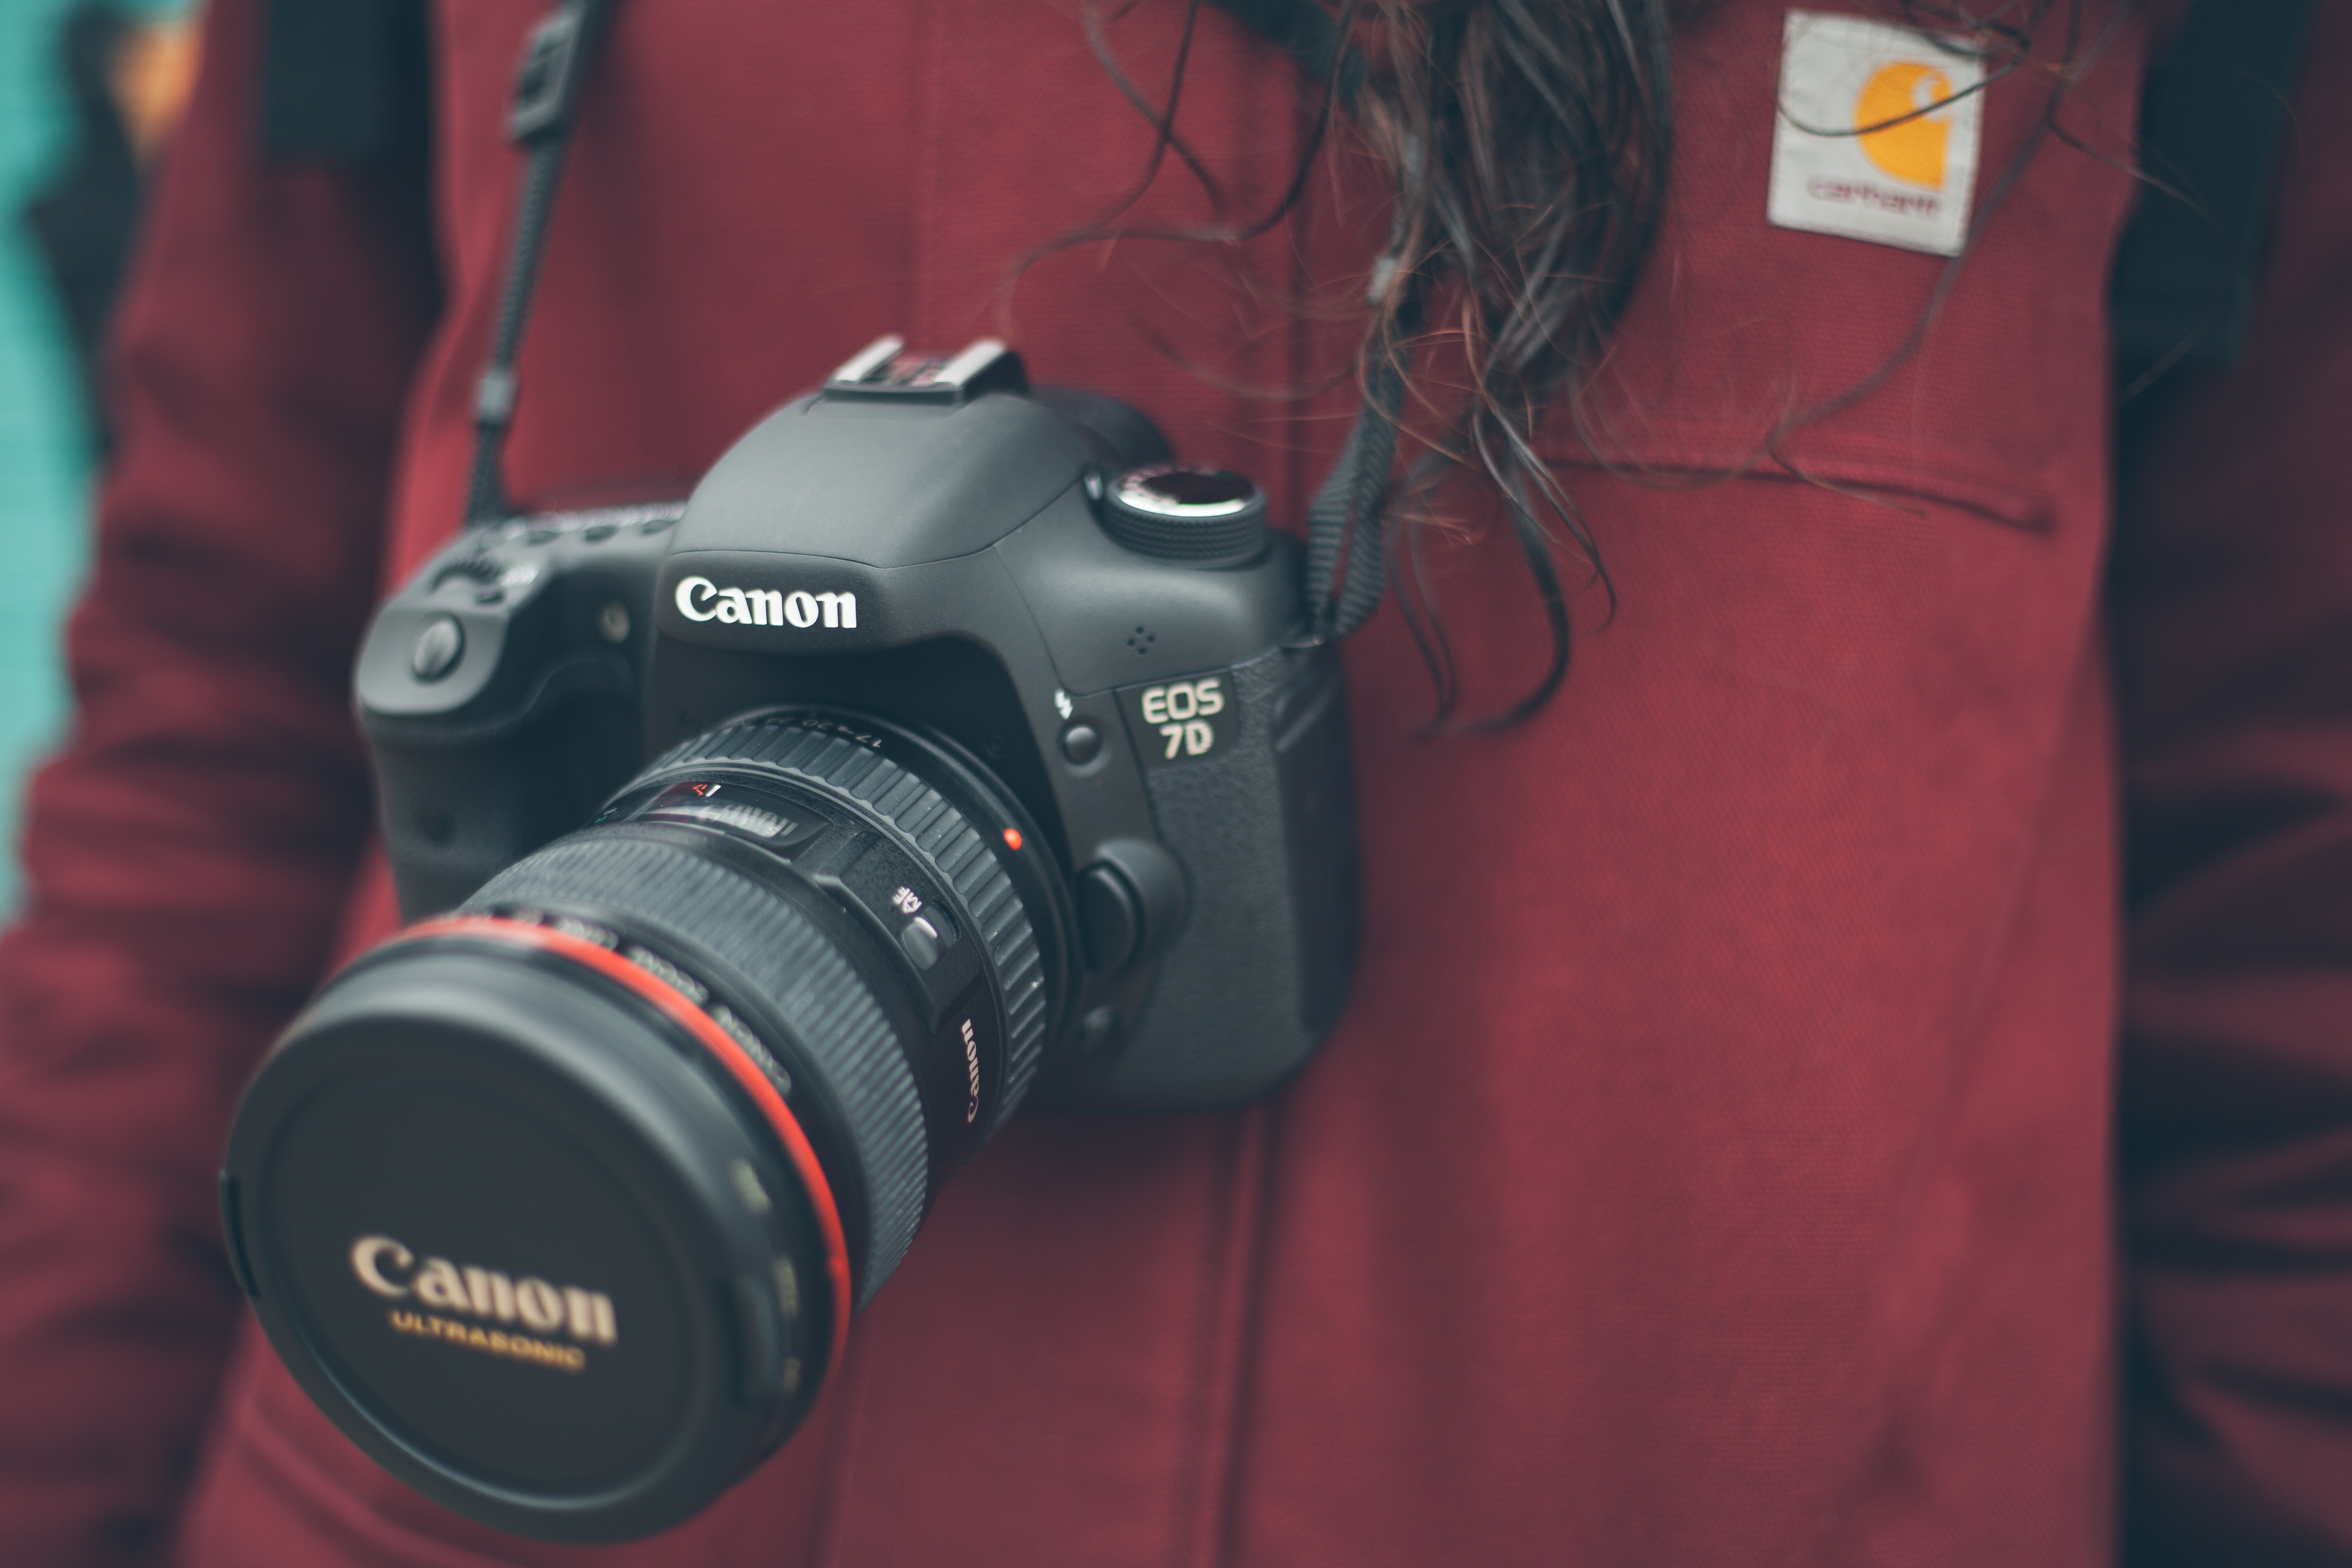
\includegraphics[width=1\textwidth]{image2.jpg}}
\end{center}


\end{appendices}
 % Anhänge

\end{document}